% !TeX spellcheck = en_GB
\documentclass[a4paper,twoside,12pt,nochapterprefix,pdftex]{scrbook}


\usepackage{amsmath,amssymb,amsthm}
\usepackage[footnotesize,sl,SL,hang,tight]{subfigure}  % helpful package for aligning figures next to each other
\usepackage{longtable} % tables over several pages
\usepackage[font={small,sl},hang,labelfont=bf]{caption} % configure captions
\usepackage{booktabs} % publication quality tables for LaTeX
\usepackage{color}
\usepackage{url}

\newcommand{\ra}[1]{\renewcommand{\arraystretch}{#1}}

\ifpdfoutput{%
	\usepackage[pdftex]{graphicx}
	\usepackage[]{pdfpages} %for including full pdf pages
}{%
	\usepackage{graphicx}
}
\usepackage{rotating} % rotate figures

\usepackage[headinclude]{scrpage2}
\usepackage[colorinlistoftodos,prependcaption,textsize=tiny]{todonotes}
%\usepackage[disable]{todonotes}
% Font packages:
\usepackage{times}
\usepackage{helvet}   % sets sans serif font
\usepackage[T1]{fontenc}

%PDF hyperref config
\ifpdfoutput{%
	\usepackage[pdftex,
		a4paper,
		bookmarks,
		bookmarksopen=true,
		bookmarksnumbered=true,
		pdfauthor={Floor Verhoeven},       % FILL THIS IN PROPERLY
		pdftitle={Sketch-based 3D Modeling in Virtual Reality},   % FILL THIS IN PRPERLY
		colorlinks,
		linkcolor=black,
		citecolor=black,
		filecolor=black,
		urlcolor=black,
		anchorcolor=black,
		menucolor=black,
		breaklinks=true,
		pageanchor=true,
		plainpages=false,
		pdfpagelabels=true]{hyperref}
}{}

\ifpdfoutput{%
	\pdfcompresslevel=9
	\pdfoutput=1
	\DeclareGraphicsExtensions{.pdf,.png}
}{}



\bibliographystyle{acmsiggraph}


% A4
%
\topmargin -0.5in
\textheight 9.3in
\textwidth 6.3in
\oddsidemargin 0.18in
\evensidemargin -0.22in
\parskip 0.1in
\parindent 0in

\renewcommand{\arraystretch}{1.5}
\renewcommand{\baselinestretch}{1}

% TO DO search symbol
\newcommand{\TODO}{\mbox{\large\bf TO DO}}
\newcommand{\REFR}{\mbox{\large\bf REFR}}

%  Terminates current page and paragraph, makes sure next page starts on
%  an odd-number, and generates a completely blank page, without page markers,
%  if necessary.
\newcommand{\clearemptydoublepage}{\newpage{\pagestyle{empty}\cleardoublepage}}


\usepackage{url}

% Stripped from acm siggraph bst and cls
\makeatletter

% no labels in bibliography.
\def\@biblabel#1{}

\newlength{\bibhang}
\setlength{\bibhang}{1em}

% Change in-bibliography biberence style
\def\thebibliography#1{%
  \section*{%
    \bibname\@mkboth{\sl\uppercase{\bibname}}{\sl\uppercase{\bibname}}}
  \list{\relax}{\setlength{\labelsep}{0em}
                \setlength{\itemindent}{-\bibhang}
                \setlength{\leftmargin}{\bibhang}}
  \def\newblock{\hskip .11em plus .33em minus .07em}
  \sloppy\clubpenalty4000\widowpenalty4000
  \sfcode`\.=1000\relax}

% Not sure what this does...
%\def\@citex[#1]#2{\if@filesw\immediate\write\@auxout{\string\citation{#2}}\fi
%  \def\@citea{}\@cite{\@for\@citeb:=#2\do
%    {\@citea\def\@citea{; }\@ifundefined
%      {b@\@citeb}{{\bf ?}\@warning
%      {Citation '\@citeb' on page \thepage \space undefined}}%
%{\csname b@\@citeb\endcsname}}}{#1}}

% Change in-document citation styles
\let\@internalcite\cite
\def\cite{\def\citename##1{##1}\@internalcite}
\def\shortcite{\def\citename##1{}\@internalcite}

\makeatother


\begin{document}

%% Define leading chapter pages
%
\addtokomafont{chapter}{\setlength{\parskip}{190pt}}   % SEVERE HACK to keep spacing to chapter art work
%\addtokomafont{chapter}{\rmfamily}        % remove this if you prefer sans-serif section titles
%\addtokomafont{section}{\rmfamily}        % remove this if you prefer sans-serif section titles
%\addtokomafont{subsection}{\rmfamily}     % remove this if you prefer sans-serif section titles
%\addtokomafont{subsubsection}{\rmfamily}  % remove this if you prefer sans-serif section titles
%\addtokomafont{paragraph}{\rmfamily}      % replace by \sffamily if you prefer sans-serif para titles
\addtokomafont{paragraph}{\sffamily}

\def\mychpstyleintl{%
{\noindent\setlength{\tabcolsep}{0pt}\setlength{\arrayrulewidth}{2pt}%
\begin{tabular}{c}
\\[100pt]
\begin{tabular}{lr}
\begin{tabular}{p{0.6\linewidth}}
\\
\end{tabular}
&
\begin{tabular}{p{0.4\linewidth}}
\rightline{{%
\sffamily%
\fontseries{bx}%
\fontshape{n}%
\fontsize{100}{120}%choose baselineskip to be 1.2 times font size
\selectfont
\thechapter}}
\end{tabular}
\end{tabular}\\[300pt]
\end{tabular}
}}

\newpagestyle{mychapterpagestyle}{{\protect\mychpstyleintl}{\protect\mychpstyleintl}}{}
\newpagestyle{myappendixpagestyle}{{\protect\mychpstyleintl}{\protect\mychpstyleintl}}{}
%%

%% macros e.g.
\newcommand{\mfytext}[0]{my fancy text}

%refs
\newcommand{\chpref}[1]{Chapter \ref{#1}}
\newcommand{\secref}[1]{Section \ref{#1}}
%\newcommand{\equref}[1]{Equation \ref{#1}} %better use builtin \eqref{}
\newcommand{\figref}[1]{Figure \ref{#1}}
\newcommand{\tabref}[1]{Table \ref{#1}}
\newcommand{\apxref}[1]{Appendix \ref{#1}}
%%

%% Replace this by your own design of a title page
%
%\title{Thesis Title}
%\author{My Name}
%\date{September 2042}
%\maketitle
%\clearemptydoublepage
% --- selfmade version ----
\begin{titlepage}
	\topmargin 1.0cm
	\oddsidemargin 0.0cm
	\evensidemargin 0.0cm
	%\textwidth 6.5in
	\centering
	\Huge
	\vspace{3.0cm}
	\textbf{\textsf{Sketch-based 3D Modeling in Virtual Reality}} \\[2.0cm]
	\includegraphics*[width=0.8\textwidth]{figures/teaser} \\ % TITLE IMAGE - replace by attractive and representative images from your thesis
	\vspace{3cm}
	\sffamily
	\Large
	Floor Verhoeven
	\\[0.8cm]
	\large
	Master Thesis
	\\
	April 2018
	\\[1.3cm]
	\emph{Supervisors:}\\
	Dr.\ Roi Poranne\\ 					% The name of the thesis supervisor
	Prof.\ Dr.\ Olga Sorkine-Hornung		% The supervising professor
	\vfill
	\includegraphics*[width=0.3\textwidth]{figures/ETH_logo} \hfill
	\includegraphics*[width=0.2\textwidth]{figures/IGL_logo}
	\vspace{3.4cm}
\end{titlepage}
\clearemptydoublepage
%%

\pagenumbering{roman}
\setcounter{page}{1}

\chapter*{Abstract}

The recent advancements in virtual reality (VR) have resulted in many new virtual reality applications. One group of applications targets 3D modeling in VR. This thesis addresses the development of a novel sketch-based 3D modeling tool in VR. Sketch-based modeling aims to provide the user with a very intuitive and simple way of creating 3D models, and is based on the way that humans draw 2D shapes with pen and paper. 

The developed system is based off the sketch-based modeling tool FiberMesh~\cite{Nealen2007} and essentially brings it to the Oculus Rift. The system is built into the mesh viewer of libigl ~\cite{Jacobson2017}, which is also ported to the Oculus Rift as part of this thesis. With our software the user can draw an outline, which will then inflate to a rough 3D model. The drawn strokes stay on the model surface and serve as deformation handles. The user can add and remove extra control curves, as well as deforming them. Finally the user can edit the mesh topology by performing cuts or extrusions. 

We show that our software is very easy to learn and intuitive, and that novice users can quickly generate 3D models with it. Also we show that this application greatly benefits from the 3D setting that comes with VR, since it allows users to do out-of-plane editing in a faster and more intuitive way. 

\todo{somewhere mention the implementation of the floor mesh in the viewer to help orientation}

\cleardoublepage


%-----------------------------------------------------------------------------------------------
%include task description here:
\cleardoublepage
%\includegraphics[viewport=3cm 0cm 20cm 27.5cm]{task_description} %better use includepdf below!
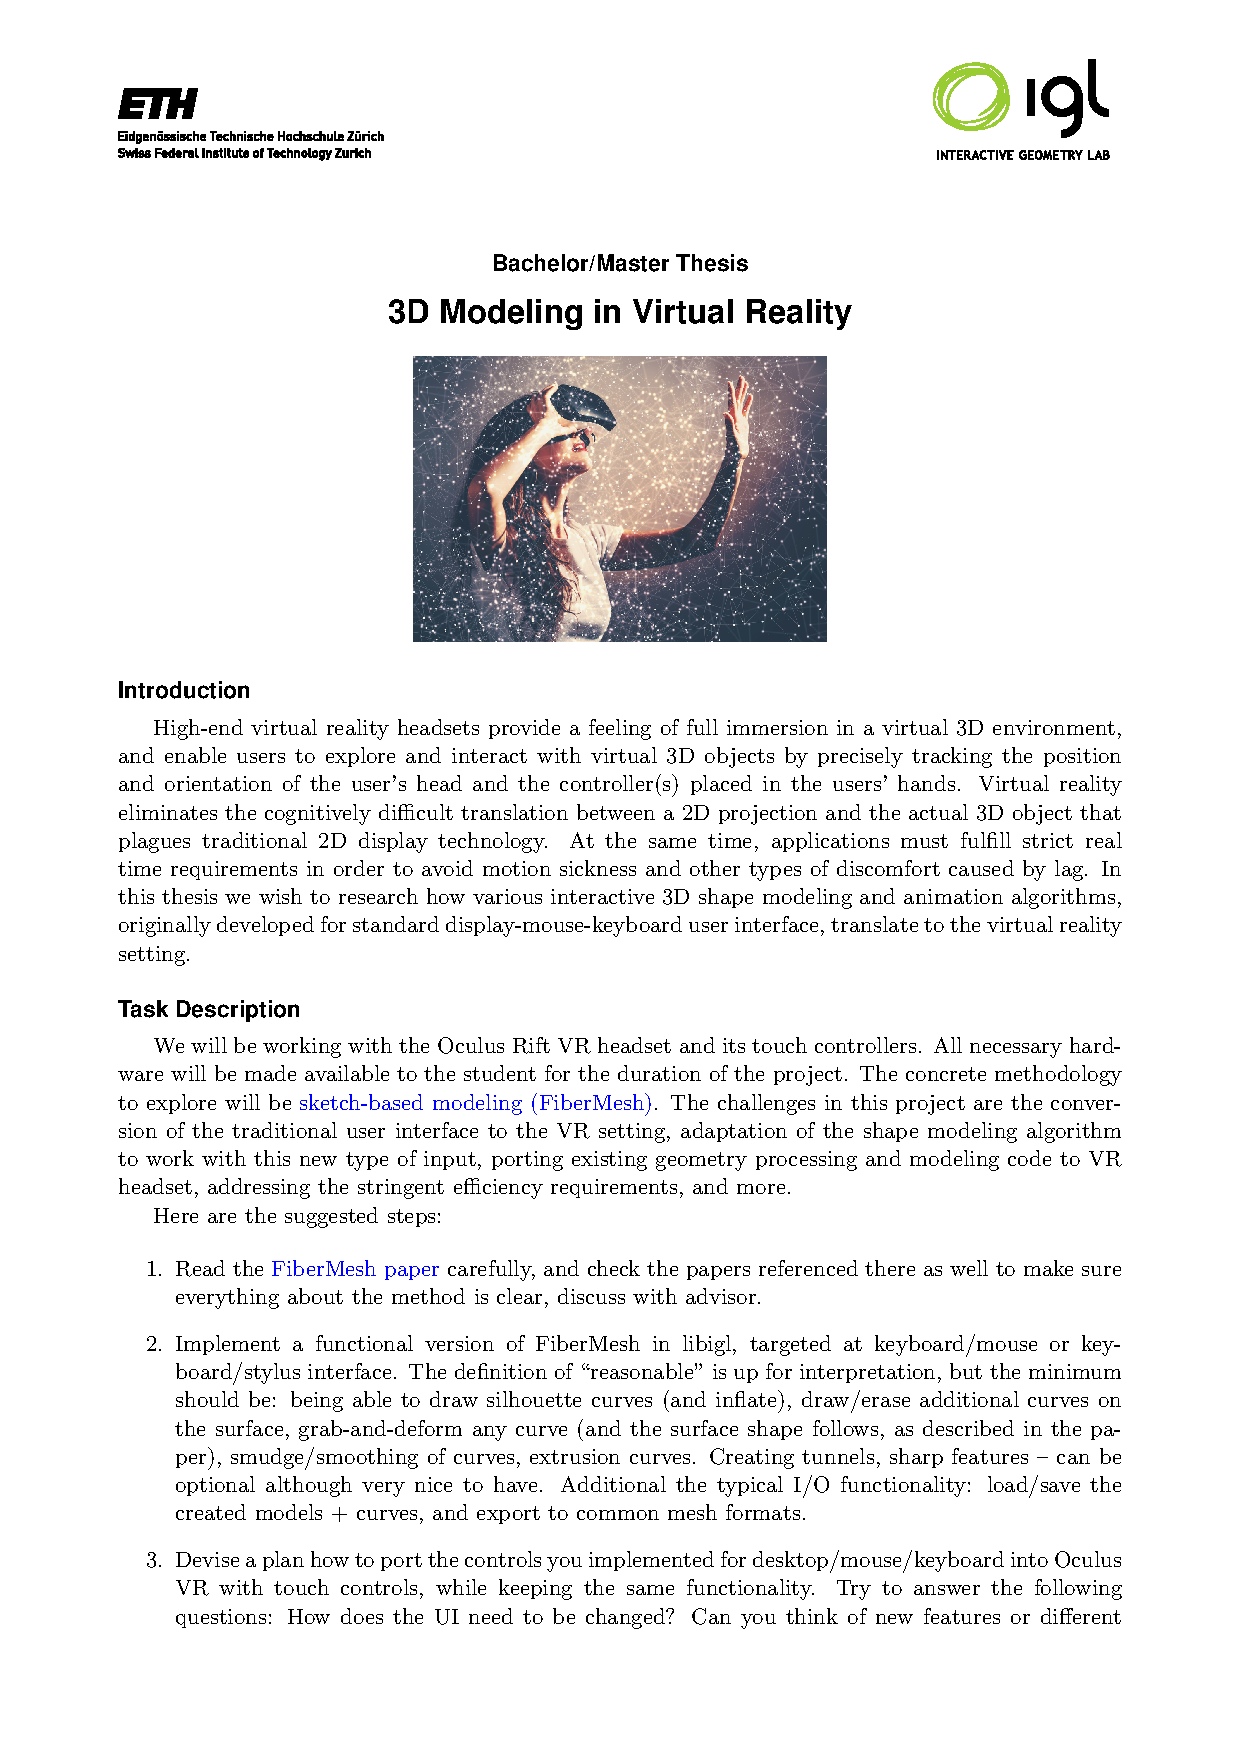
\includepdf[pages={1,2}]{Thesis_task_description}
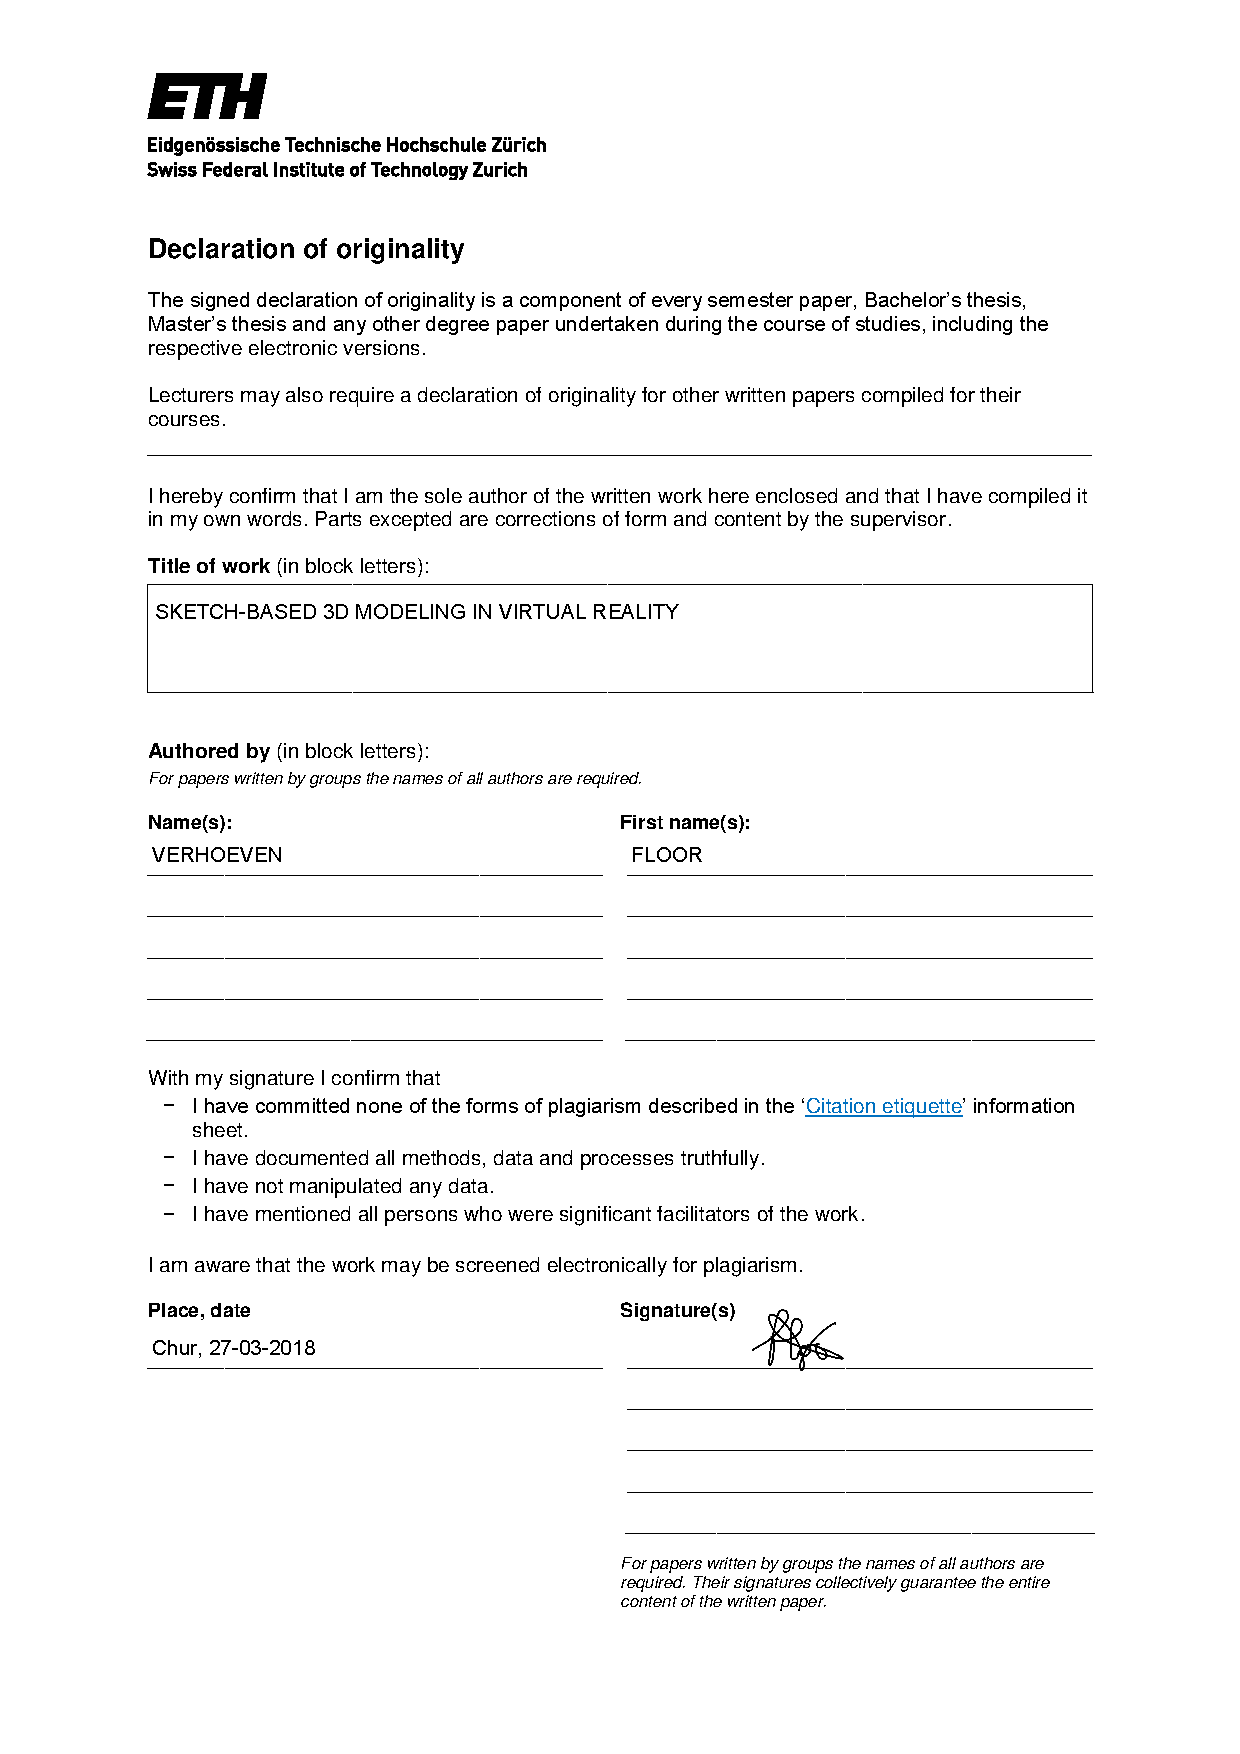
\includepdf{declaration-originality}
\cleardoublepage
%-----------------------------------------------------------------------------------------------

%include acknowledgment here:
%\include{acknowledgment}

\tableofcontents

\cleardoublepage
\phantomsection
\addcontentsline{toc}{chapter}{List of Figures}
\listoffigures

\cleardoublepage
\phantomsection
\addcontentsline{toc}{chapter}{List of Tables}
\listoftables
\cleardoublepage

\pagenumbering{arabic}
\renewcommand*{\chapterpagestyle}{mychapterpagestyle}
\renewcommand*{\chapterformat}{} % show chapter titles only (no numbers)
% \setchapterpreamble[o]{...}  unfortunately does not move the \chapter output downwards

% ---- MAIN PART ----

% set counter to n-1:
\setcounter{chapter}{0}

\chapter{Introduction}
Digital 3D shape modelling is a field that has received a lot of attention over the past years as a result of increasing rendering possibilities and a growing call for digital content. The recent surge in interest for VR (Virtual Reality) has driven the development of better GPUs (Graphics Processing Unit) even more, while also further increasing the demand for digital 3D content. 
The process of 3D shape modelling has so far been almost exclusively suitable for trained professionals or users with a lot of experience. While 3D modelling software generally comes with plenty of options and possibilities it also usually has a steep learning curve. This causes 3D modelling to become inaccessible to novice users who would like to develop some 3D content, but who do not have the time to learn how to use these programs. 

Sketch-based 3D modelling seeks to simplify the process of 3D modelling in order to make it more accessible to this user group. Its goal is to provide the user with intuitive ways to interact with the mesh that is being modelled. Previous work regarding sketch-based modelling tools has produced multiple software products which  present the user with this intuitive method of 3D modelling. 

Recently a variety of art creation tools for usage in VR have been created. These applications range from painting in 3D to voxel modelling and 3D sculpting. VR gives artists the possibility to look at what they're creating from a literally new perspective. Directly modelling in 3D gives a better feeling of the proportions of different parts of a model and for example the angles between them.
\todo{insert screenshots of existing software / models}

The goal of this thesis is to develop a sketch-based 3D modelling program for usage in VR. This combines the intuitivity of sketch-based designing and the emersiveness of modelling in actual 3D space and the possibility of viewing the results immediately in 3D. The software is targeted to user that are new to 3D modelling and should therefore be straightforward to use and easy to learn.
% set counter to n-1:
%\setcounter{chapter}{1}

\chapter{Related Work}
\label{chap:related}
A lot of software for the purpose of 3D modelin exists, with some of the best known ones being Maya, Blender, Autodesk 3ds Max and Zbrush~\cite{Maya, Blender, 3dsMAX, ZBrush}. Typically these software let their users manipulate meshes on vertex, edge or face level, resulting in very fine-grained control over the appearance of created models. Although this makes these programs very powerful and versatile for the creation and editing 3D models, they come with a very steep learning curve and are overcomplete for recreational users. This chapter instead focusses on describing some of the more intuitive and easy-to-use sketch-based 3D modeling software, as well as a couple of relatively new software for creating 3D content in VR. 

\section{Sketch-based Modeling}
Sketch-based modeling is a modeling technique that aims to transfer the way that people draw shapes with pen and paper to a method of modeling 3D shapes on the PC with a mouse. With the mouse the user draws strokes on the screen, whose interior is subsequently meshed and then inflated to smooth rotund 3D meshes. Typically the user can then edit this initial mesh by specifying additional strokes that for example create extrusions or cut the mesh.
The software that was written as part of this thesis also adopts the sketch-based modeling paradigm. 


\subsection{FiberMesh}
\label{subsec:fiber}
FiberMesh is a system that allows modeling freeform surfaces by drawing 3D curves~\cite{Nealen2007}. The user-defined curves are used to create a 3D model and stay present on the model and can be used to edit the geometry. This allows for a very intuitive method of deforming and editing meshes after their initial creation. FiberMesh lets users define curves as smooth or sharp, add and remove control curves on the mesh and pull curves to deform the mesh. Additionally it allows the user to change the mesh topology by cutting parts of the mesh and creating extrusions or tunnels.

Algorithmically FiberMesh depends on two main steps, namely curve deformation and surface optimization. In addition to these two steps, there are also a mesh construction and remeshing step, which only occur after new mesh topology has been created (e.g.\ after creation, cut or extrusion). 

For curve deformation they used a detail-preserving deformation method that combines differential coordinates~\cite{Sorkine2006} with co-rotational methods~\cite{Felippa2007}. A sequence of linear least-squares problems is solved, while satisfying the user-defined positional constraints on the drawn curves. The rotation matrices are explicitly represented as free variables, as they cannot be derived from the curves which are nearly collinear. In order to accommodate for large linear  rotations, the gross rotation is computed by iteratively concatenating small delta rotations that are each obtained by solving a linear system. The linear system that is solved in each step can be seen in equation \ref{eq:1}.  

\begin{equation} \label{eq:1}
	\arg\min_{\mathbf{v, r}} \left\lbrace \sum_{i} \left\Vert \mathbf{L}\left(\mathbf{v}_{i}\right) - \mathbf{r}_{i}\mathbf{R}_{i}\mathbf{\delta}_{i}\right\Vert^{2} + \sum_{i \in C_{1}} \left\Vert \mathbf{v}_{i} - \mathbf{v}_{i}^{'} \right\Vert^{2} + \sum_{i,j \in E}	 \left\Vert \mathbf{r}_{i}\mathbf{R}_{i} - \mathbf{r}_{j}\mathbf{R}_{j} \right\Vert^{2}_{F} + \sum_{i \in C_{2}} \left\Vert \mathbf{r}_{i}\mathbf{R}_{i} - \mathbf{R}_{i}^{'} \right\Vert^{2}_{F} \right\rbrace 
\end{equation}

Here $\mathbf{L}(\cdot)$ is the differential operator, $\mathbf{v}_{i}$ is the coordinates of vertex i, $\Vert \cdot \Vert_{F}$ is the Frobenius norm, $E$ is the set of curve edges and $C_{1}$ and $C_{2}$ are the sets of constrained vertices, primed values are constraints, $\mathbf{R}_{i}$ represents the gross rotation (in the deformed curve) corresponding to vertex i obtained from the previous iteration, and finally $\mathbf{r}_{i}$ is a linearized incremental rotation for vertex i given by a skew symmetric matrix with 3 unknowns,

\begin{equation*}
\mathbf{r}_{i} = \left[ \begin{matrix}
1 & -r_{iz} & r_{iy} \\
r_{iz} & 1 & -r_{ix} \\ 
-r_{iy} & r_{ix} & 1
\end{matrix} \right].
\end{equation*}

Rotations are updated by setting them to $\mathbf{R}_{i} = \mathbf{r}_{i}\mathbf{R}_{i}$ and orthonormalizing the result using polar decomposition~\cite{Fu2007}.
In the iterative process of estimating rotations, they use first order differentials ($L_0$), and for computing the final vertex positions using this estimated rotations they use the second order differential ($L_1$). 

\begin{equation*}
L_{0} = \mathbf{v}_{i} - \mathbf{v}_{i-1}, \quad L_{1} = \mathbf{v}_{i} - \frac{1}{\lvert N_{i} \rvert} \sum_{j \in N_{i}} \mathbf{v}_j.
\end{equation*}

For surface optimization, FiberMesh solves 3 sparse linear systems in order to compute a smooth mesh surface that adheres to the user-defined constraint curves. The first system solves for a set of smoothly varying Laplacian magnitudes $\{c_{i}\}$ which approximate the scalar mean curvature values. The least-squares minimization that it solves is as follows: 

\begin{equation}
\arg\min_{c} \left\lbrace \sum_{i} \left\Vert \mathbf{L}\left(c_{i}\right) \right\Vert^{2} + \sum_{i} \left\Vert c_{i} - c_{i}^{'} \right\Vert^{2} \right\rbrace
\end{equation}

Where $\mathbf{L\left(\cdot\right)}$ denotes the discrete graph Laplacian, which is independent of the exact mesh geometry, allowing us to reuse it in multiple iterations.
In the first iteration, the target Laplacian magnitudes are only set for the constrained curves by using the scalar mean curvature along the curve. 

To obtain a geometry that satisfies these target Laplacian magnitudes, Nealen et al.\ use the uniform Laplacian as an estimator of the integrated mean curvature normal, which is computed by $\delta_{i} = A_{i} \cdot c_{i} \cdot \mathbf{n}_{i}$, where $A_{i}$ is an area estimate for vertex i, $c_{i}$ is the target Laplacian magnitude and $\mathbf{n}_{i}$ is the estimated normal from the current face normals. However the uniform Laplacian is not an accurate estimator of the integrated mean curvature normal when the incident edges to a vertex are not of equal length. To solve for this problem without using a geometry dependent discretization and thus avoiding recomputing the matrix for every iteration, they prescribe target edge vectors in an attempt to achieve equal edge length. This is done by solving the following linear system (which uses the same matrix as the system that solves for target Laplacian magnitudes) to obtain a smooth set of target average edge lengths $e_{i}$: 

\begin{equation}
\arg\min_{e} \left\lbrace \sum_{i} \left\Vert \mathbf{L}\left(e_{i}\right) \right\Vert^{2} + \sum_{i} \left\Vert e_{i} - e_{i}^{'} \right\Vert^{2} \right\rbrace
\end{equation}

Again the first iteration is performed with only the edge lengths along the constrained curve. 
The target average edge lengths are then used to compute target edge vectors for a subset $B$ of mesh edges (in the first iteration this subset only contains edges along the constrained curves, and afterwards it contains all edges incident to the constrained curves) as follows:
\begin{equation}
\eta_{ij} = \left( e_{i} + e_{j} \right) / 2 \cdot \left( \mathbf{v}_{i} - \mathbf{v}_{j} \right) / \left\Vert \mathbf{v}_{i} - \mathbf{v}_{j} \right\Vert.
\end{equation}

These target edge vectors are then used to solve a linear system that gives the updated vertex positions as follows: 

\begin{equation}
\arg\min_{\mathbf{v}} \left\lbrace \sum_{i} \left\Vert \mathbf{L}\left(\mathbf{v}_{i}\right) - \delta_{i} \right\Vert^{2} + \sum_{i \in C} \left\Vert \mathbf{v}_{i} - \mathbf{v}_{i}^{'} \right\Vert^{2} + \sum_{\left(i,j\right) \in B} \left \Vert \mathbf{v}_{i} - \mathbf{v}_{j} - \eta_{ij} \right\Vert^{2} \right\rbrace
\end{equation}

The systems for solving for target Laplacian magnitudes, average edge lengths and optimal vertex positions are solved iteratively until convergence (approximately 5-10 iterations). Since only a geometry independent discretization of the Laplacian is used, the system matrix can be reused between iterations, until the mesh topology is changed (for example by a cutting action). Because of this, the slow matrix factorization only needs to happen once for a given mesh topology, resulting in a fast algorithm that allows for interactive rates.	

\section{3D Modeling in Virtual Reality}
\label{sec:3dmodeling}
Over the last couple of years, plenty of VR applications have been published that involve creating some type of digital 3D content. The software can roughly be split into 2 categories, namely for creating 3D paintings and for creating 3D models (assembled from a structure of vertices, edges and faces). Whereas the former category focusses on the artistic side of 3D content and usually does not result in work that can be exported to some standard format, the latter category more aims to provide a tool for producing 3D models that can be exported and then used in some other VR or 3D application. 
This section describes a variety of these 3D virtual reality applications, their interfaces and what kind of content users can make with them. 

\subsection{Google Tilt Brush}
Google's Tilt Brush is available for the Oculus Rift and HTC Vive and allows the user to  create room-scale art in the style of 3D paintings. The software provides different types of tools and brushes, including special effects tools like a fire or stars brush. Users cannot export their creations to typical model formats such as .obj or .off, but they can turn them into a GIF or upload them to Google Poly where other users can explore and enjoy their work.
Figure~\ref{fig:tiltart}~(a) shows a screenshot of example 3D artwork that has been made with Google Tilt Brush (the original work has stars that change their light intensity and seem to twinkle). In order to give the user easy access to the large set of different painting tools, Tilt Brush has created an embedded menu in the form of a painters palette that is attached to the controller in the user's non-dominant hand. Several of the menus allow for browsing through further submenus. The dominant hand is used to select a tool from the menu and paint with it. Figures~\ref{fig:tiltart}~(b) and~\ref{fig:tiltart}~(c) show two examples of what the hand-held palette menus looks like and you can see that the user can twist his hand in order to view more menu options on the backside of the palette.

\begin{figure}[t!]
    \centering
    \setlength{\tabcolsep}{0.0130\linewidth}
    \begin{tabular}{@{}c@{}}
    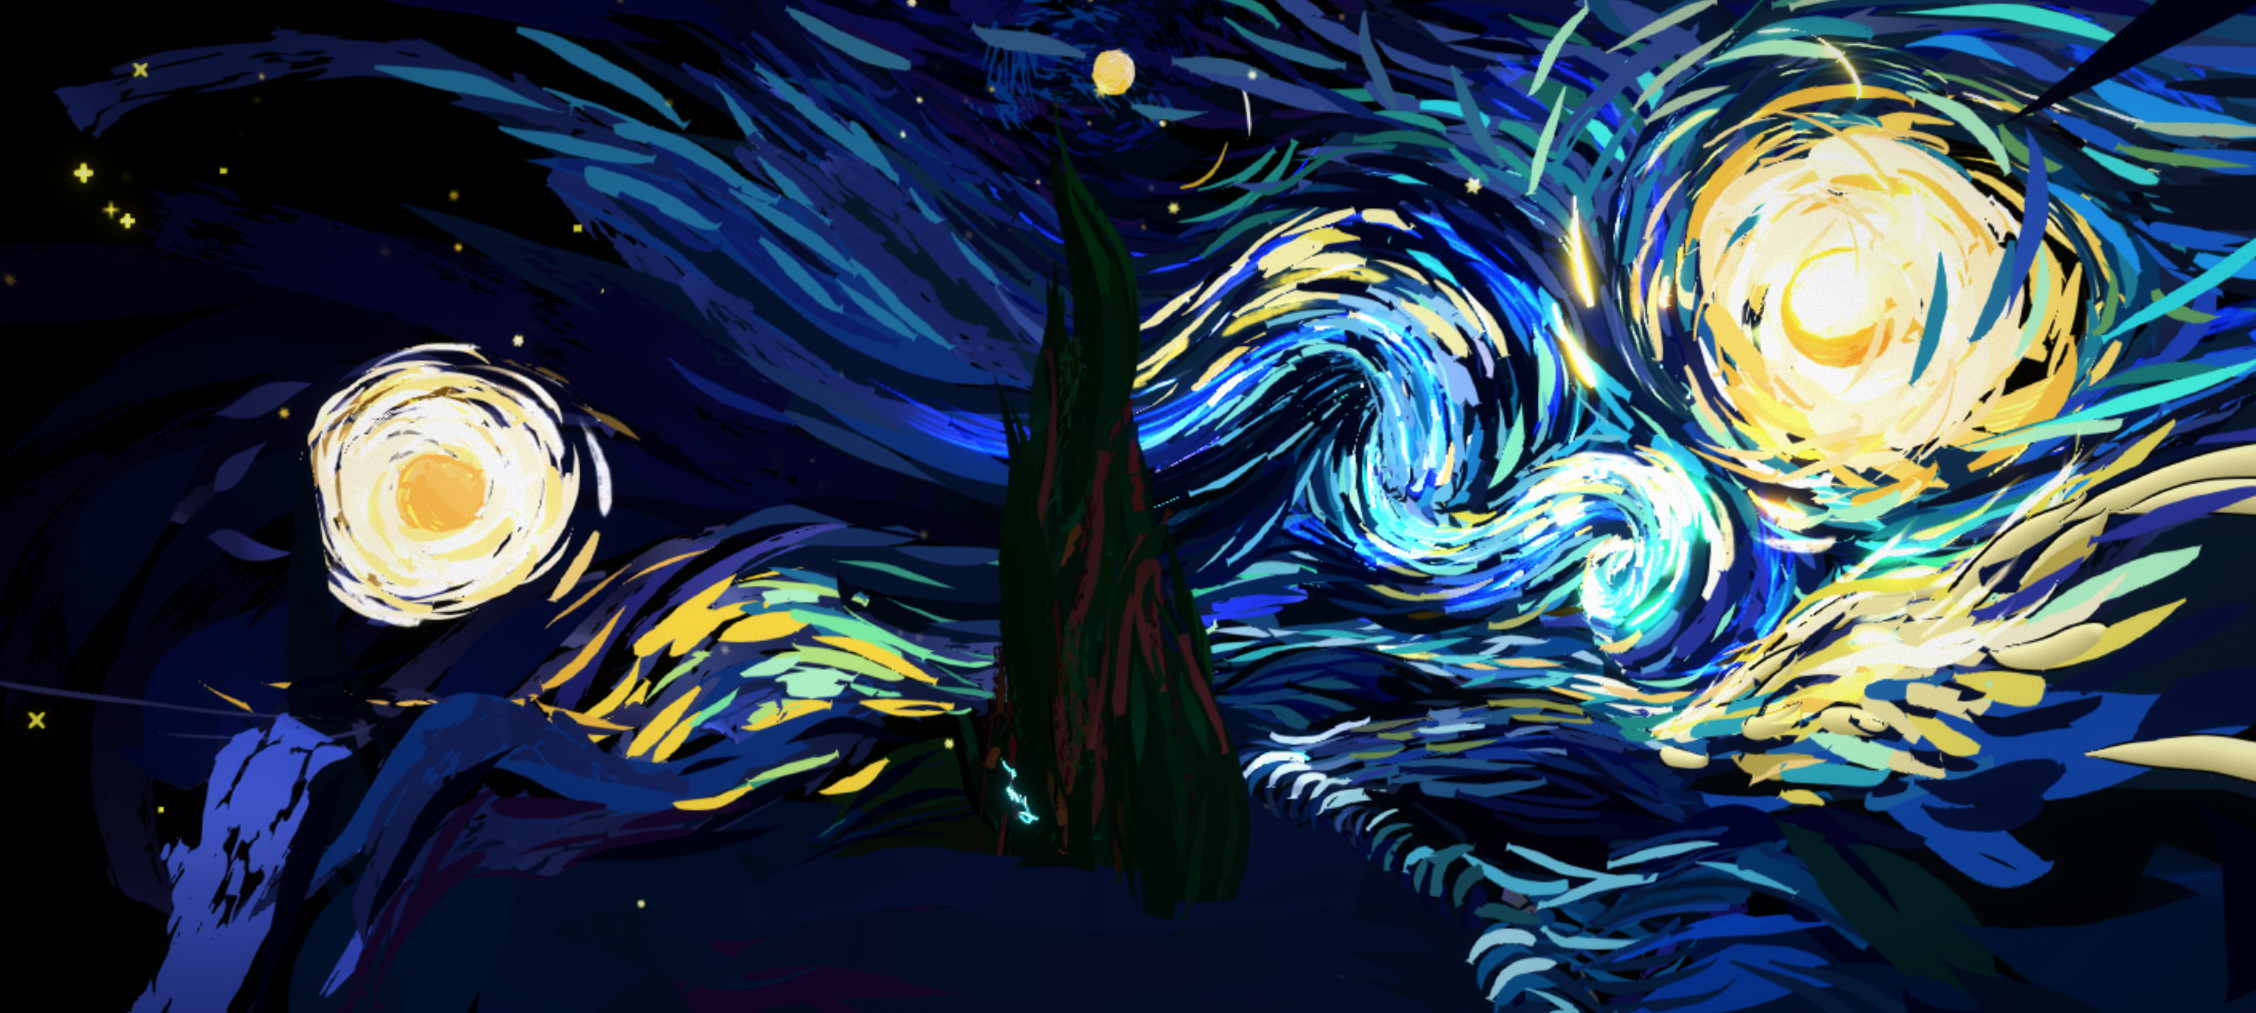
\includegraphics[width=0.7260\linewidth]{figures/TiltBrush_StarryNight}\\
    (a)
    \end{tabular}
    
    \centering
    \setlength{\tabcolsep}{0.0130\linewidth}
    \begin{tabular}{@{}cc@{}}
   	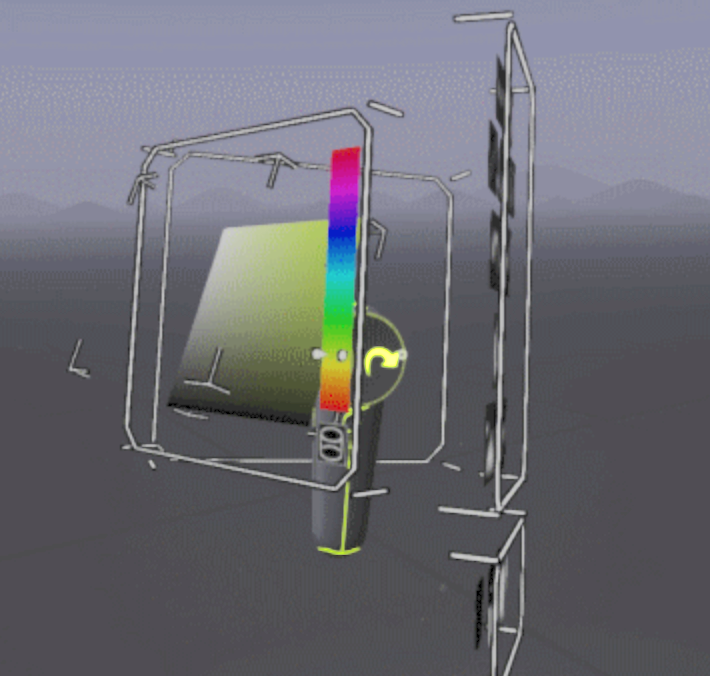
\includegraphics[width=0.35\linewidth]{figures/Tilt_menu2}&
    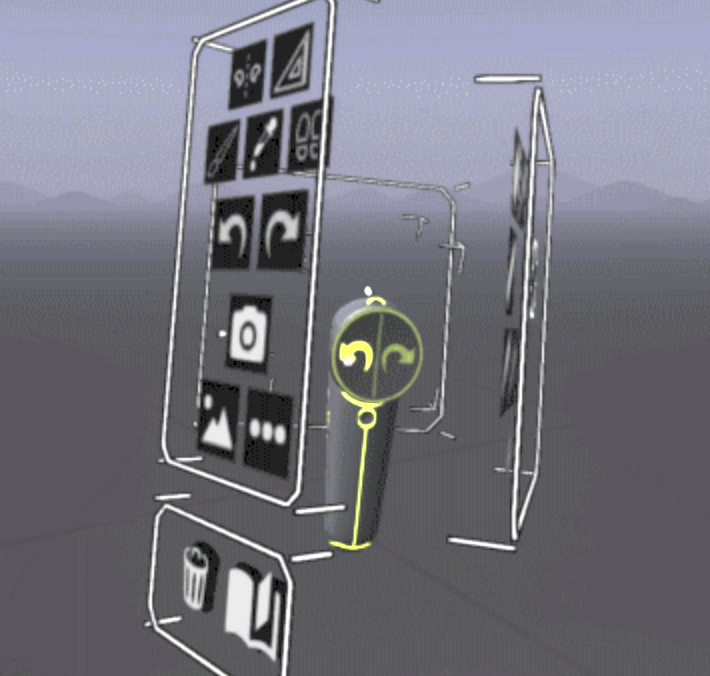
\includegraphics[width=0.35\linewidth]{figures/Tilt_menu1}\\
    (b)&(c)\\
    \end{tabular}
    \caption[Google Tilt Brush]{Google Tilt Brush.
    	  \textup{(a)} Recreation of Van Gogh's Starry Night (moving version available at https://poly.google.com/view/e-Zqenw7Dui).
			  \textup{(b)} Left-side view of the "hand-held" user interface of Google Tilt Brush. \textup{(c)} Right-side view of the "hand-held" user interface of Google Tilt Brush.
      \label{fig:tiltart}}
\end{figure}

\subsection{Oculus Medium}
Oculus Medium is a 3D sculpting tool that is only available for the Oculus Rift. Conceptually the user can paint with volumetric brushes, much like sculpting with clay. For instance the user will draw a simple circle and this will result in a donut shape. With several tools the user can sculpt away or add extra clay, as well as assigning multiple colors to the surface.
Unlike Google Tilt Brush, Oculus Medium does allow the user to store created models in .obj format, so they can be exported for use in other programs. The interface is quite intuitive since it shows a very strong connection to the method of creating 3D shapes with the use of clay in real life which most users have experience with. Users can quickly create rough shapes and refine them by adapting the brush size and adding small-scale details. The dominant hand of the user serves as the so-called "Tool hand" which can be used to sculpt with, while the non-dominant hand serves as the "Support hand" which can be used to open up several hand-held menus. Figures~\ref{fig:medium}~(a) and~\ref{fig:medium}~(b) show examples of complicated 3D models that have been made in Oculus Medium. One of the unique features of Oculus Medium is the functionality to create and use stamps, which helps easily create interesting textures on the models like the fur and grass in Figure~\ref{fig:medium}~(a).


\begin{figure}[!h]
    \centering
    \setlength{\tabcolsep}{0.0130\linewidth}
    \begin{tabular}{@{}cc@{}}
    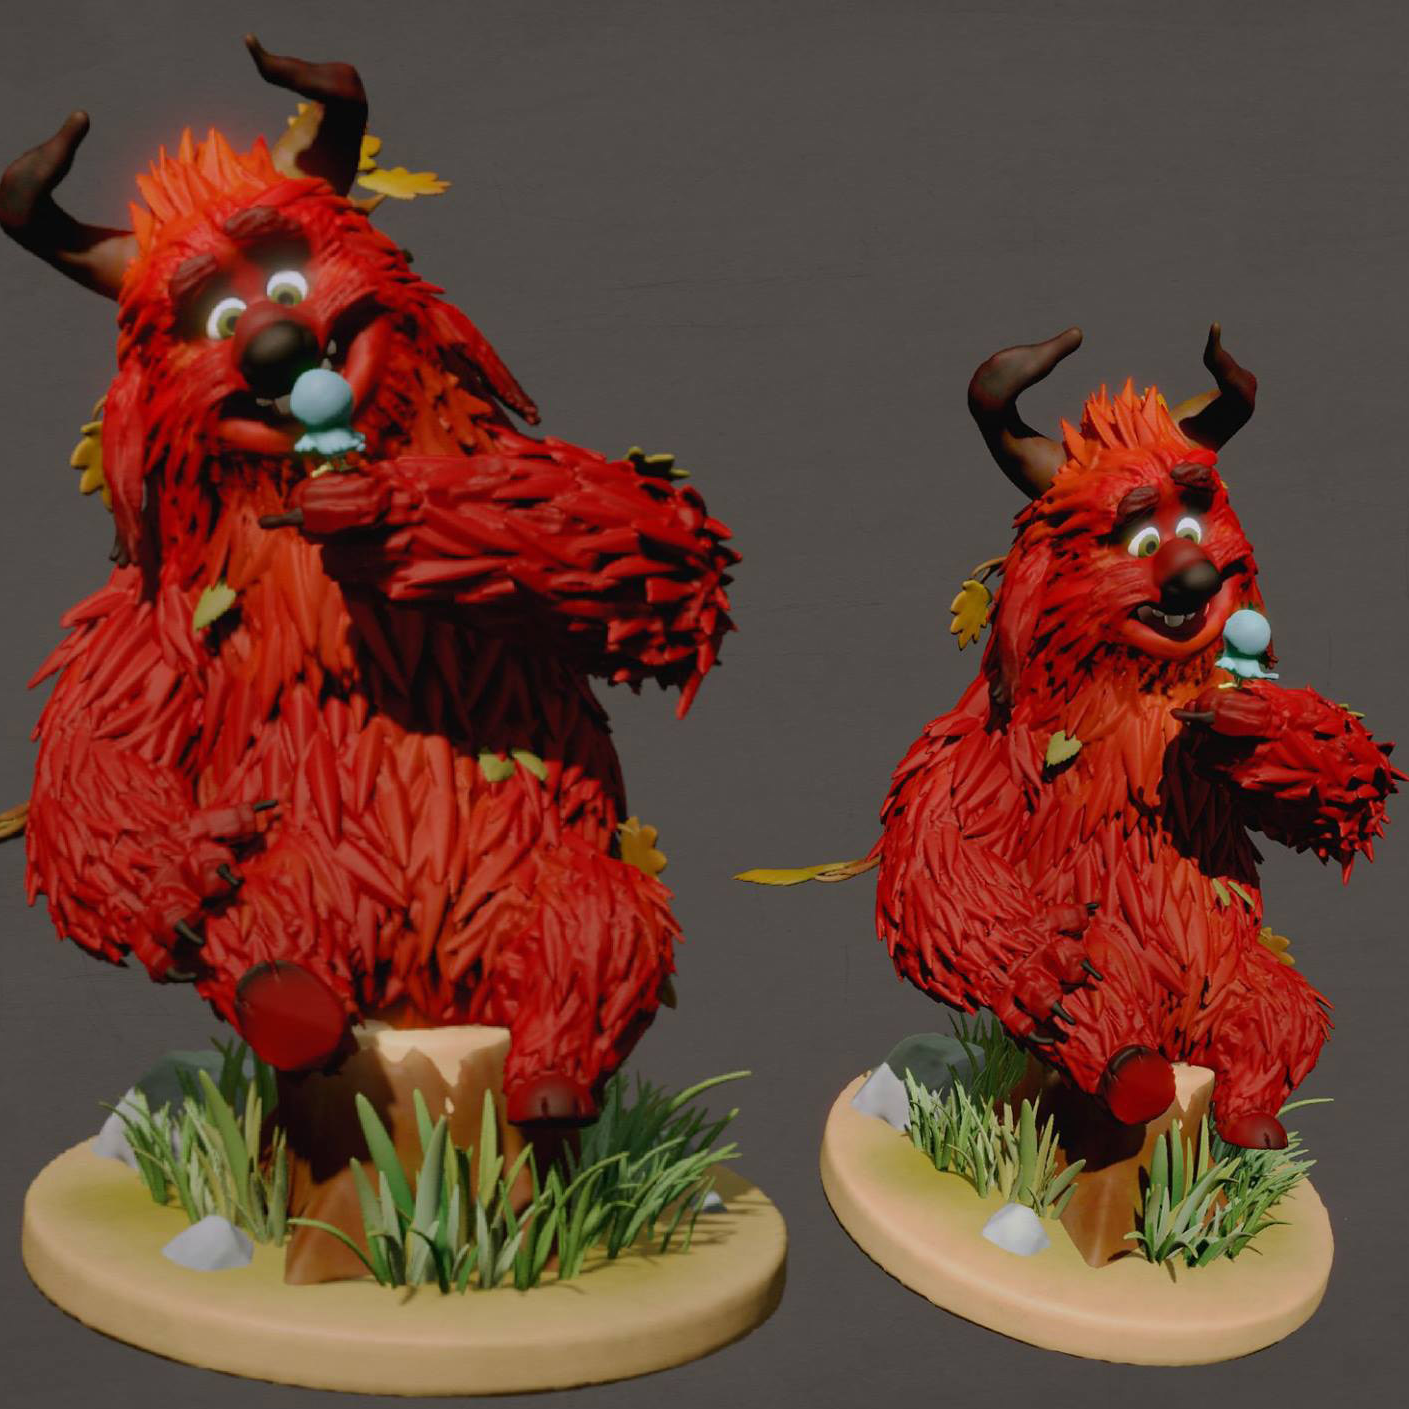
\includegraphics[width=0.35\linewidth]{figures/medium_goro_fujita} &
    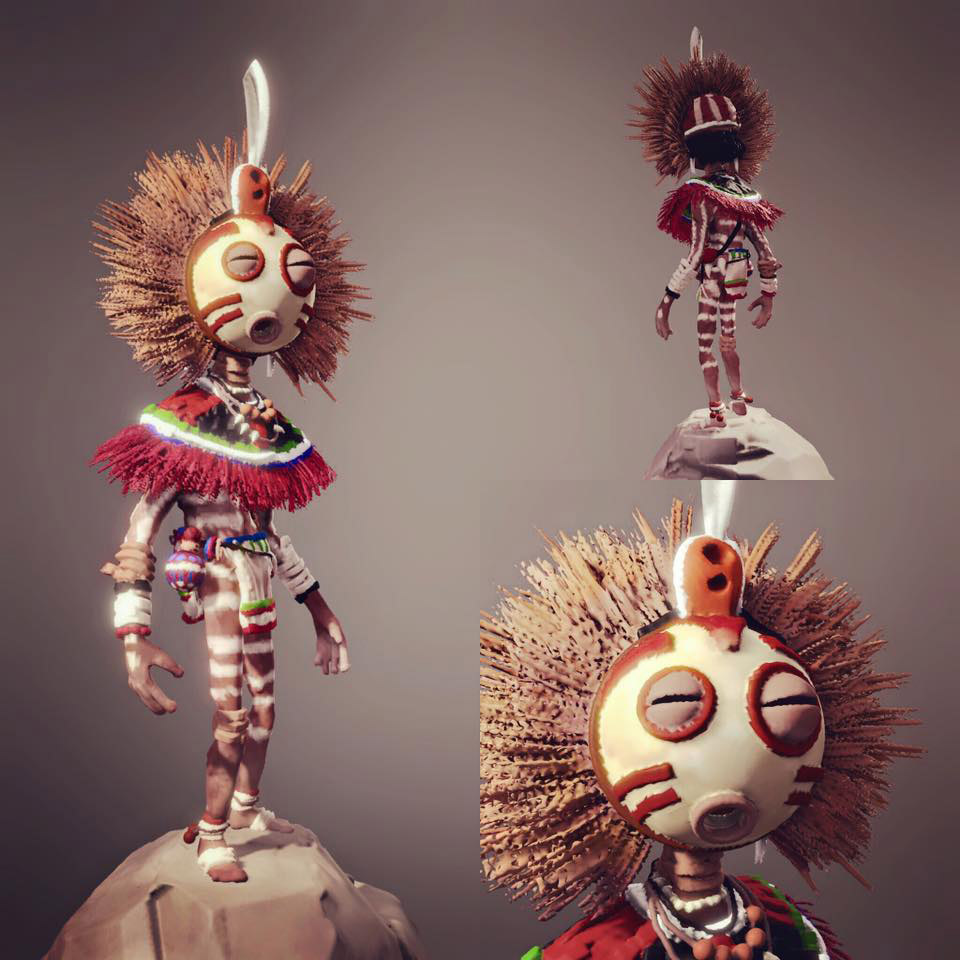
\includegraphics[width=0.35\linewidth]{figures/medium_goro_fujita2}\\

    (a)&(b)\\
    \end{tabular}
    
    \centering
    \setlength{\tabcolsep}{0.0130\linewidth}
    \begin{tabular}{@{}cc@{}}
   	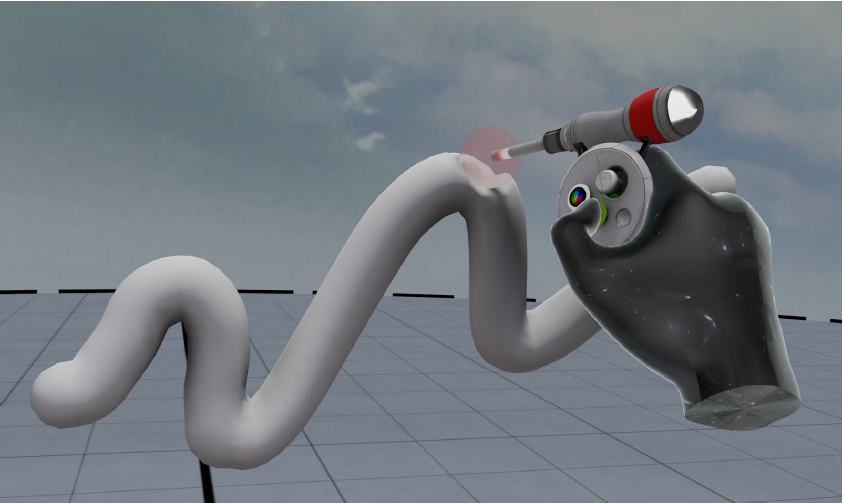
\includegraphics[width=0.35\linewidth]{figures/medium_interface1}&
   	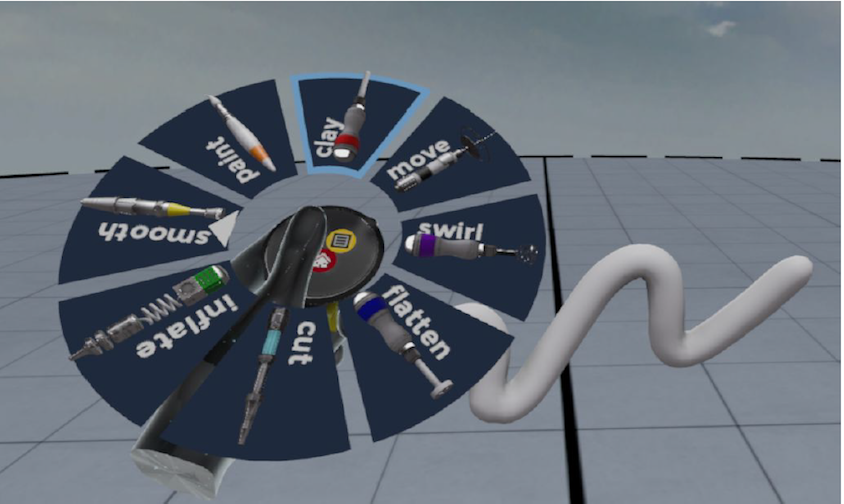
\includegraphics[width=0.35\linewidth]{figures/medium_interface2}\\
    (c)&(d)\\
    \end{tabular}
    \caption[Oculus Medium]{Oculus Medium.
    	  \textup{(a)} Model of a furry monster created in Oculus Medium by artist Goro Fujita.
			  \textup{(b)} Model of an African figure created in Oculus Medium by artist Goro Fujita. \textup{(c)} Sculpting view in Oculus Medium. \textup{(d)} Menu view in Oculus Medium.
      \label{fig:medium}}
\end{figure}

\subsection{MasterpieceVR}
MasterpieceVR brings a combination of the design paradigms used by Oculus Medium and Google Tilt Brush, letting the user mix volume sculpting with 3D painting. It is available for Oculus Rift, HTC Vive and Windows Mixed Reality, and for each of them it requires the accompanying controllers for input. One of MasterpieceVR's biggest selling points is that it allows multiple users to work on one model simultaneously, allowing interactive collaboration with direct feedback between artists. Like Oculus Medium, MasterpieceVR lets the user export models (including vertex colors) to .obj, as well as .fbx format. Additionally, users can load reference images or models into the program, which can greatly simplify modeling. MasterpieceVR implements menus in a similar fashion to Google Tilt Brush and Oculus Medium, with a menu of icons held in the user's non-dominant hand. Compared to these two, MasterpieceVR however has a larger and less intuitive menu layout. Figure~\ref{fig:masterpieceVR}~(a) shows a complex model created in MasterpieceVR and Figure~\ref{fig:masterpieceVR}~(b) shows the menu interface.

\begin{figure}[!h]
    \centering
    \setlength{\tabcolsep}{0.0130\linewidth}
    \begin{tabular}{@{}cc@{}}
   	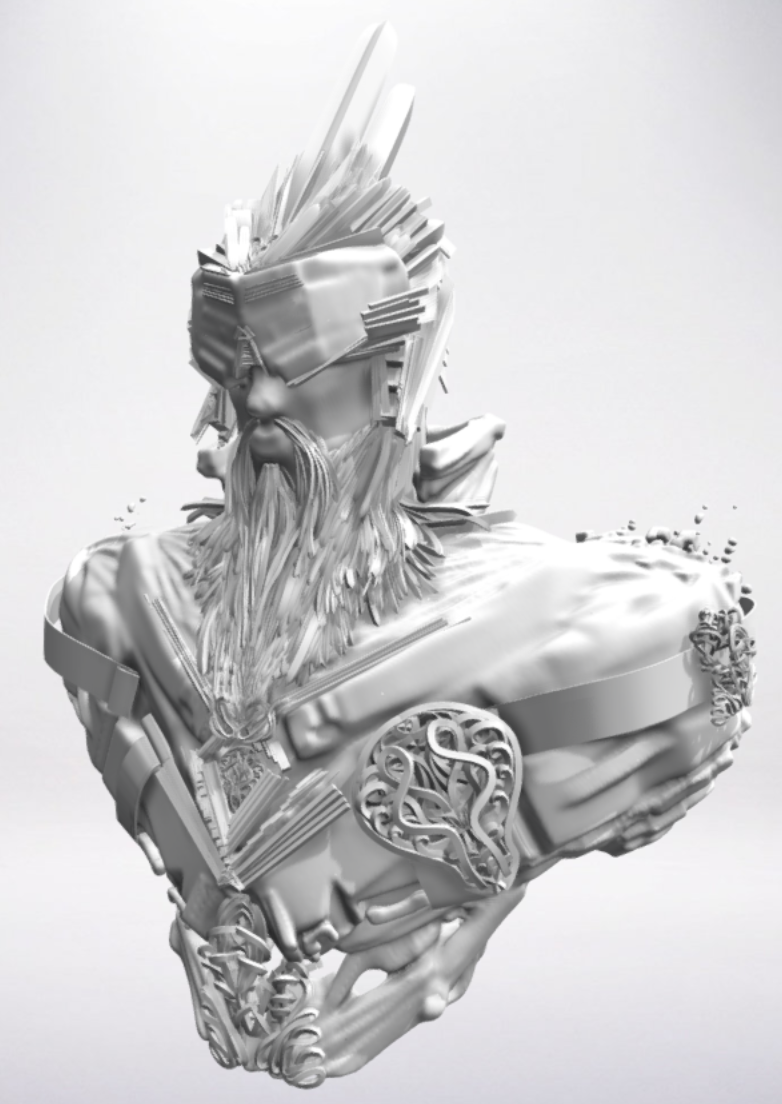
\includegraphics[width=0.35\linewidth]{figures/MasterpieceVR_Vladimir_Ilic}&
   	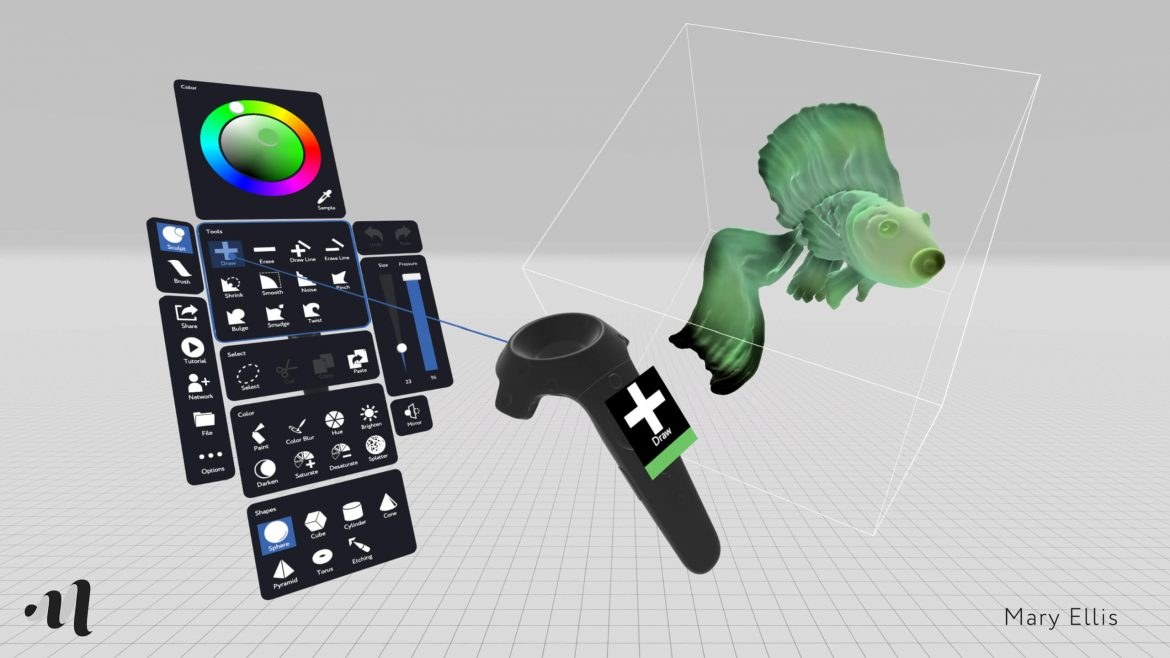
\includegraphics[width=0.5\linewidth]{figures/MasterpieceVR_interface}\\
    (a)&(b)\\
    \end{tabular}
    \caption[MasterpieceVR]{MasterpieceVR.
    	  \textup{(a)} Model of a warrior created in MasterpieceVR by artist Vladimir Ilic.
			  \textup{(b)} Interface of MasterpieceVR (model by Mary Ellis). 
      \label{fig:masterpieceVR}}
\end{figure}

\subsection{Google Blocks}
Google Blocks is available for Oculus and HTC Vive and is Google's software for creating 3D objects in VR. From the programs mentioned in this section, Google Blocks seems the most similar to professional non-VR based modeling software like Blender~\cite{Blender} or Maya~\cite{Maya}. Users can start with several predefined shapes like spheres, cubes or cones and can edit the models on face, edge or vertex level. While this gives the user a lot of artistic freedom and extra modeling possibilities, it also makes its usage a lot less intuitive than the other VR 3D modeling software that is available. Although the user has low-level control, the created meshes are very low-poly compared to the models created with for example Oculus Medium. The user does not have control over the number of polygons, which results in less realistic and smooth models. Again the created models can be exported as .obj file. Figures~\ref{fig:blocks}~(a) and~\ref{fig:blocks}~(b) show a simple model of an anglerfish created in Google Blocks, and the simple Google Blocks interface.

\begin{figure}[!h]
    \centering
    \setlength{\tabcolsep}{0.0130\linewidth}
    \begin{tabular}{@{}cc@{}}
   	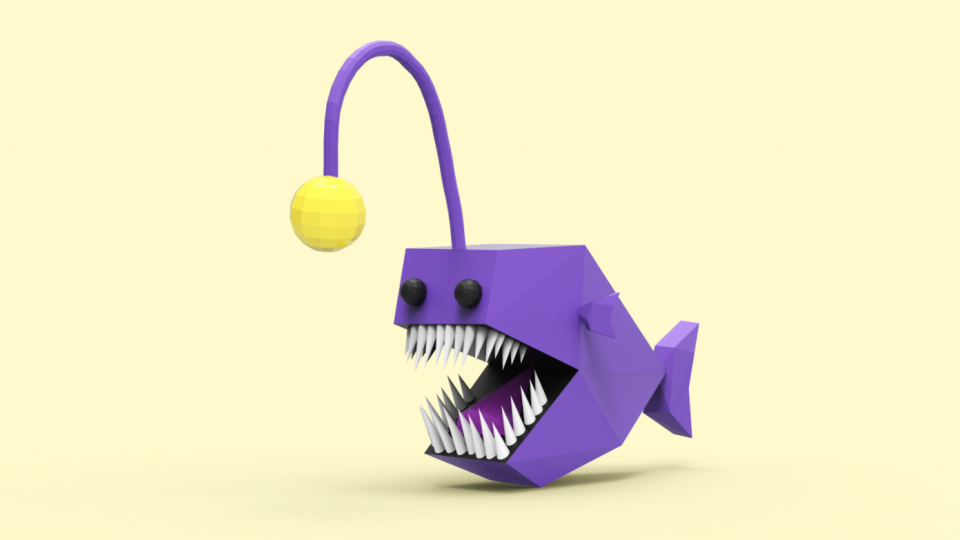
\includegraphics[width=0.487\linewidth]{figures/blocks_anglerfish}&
   	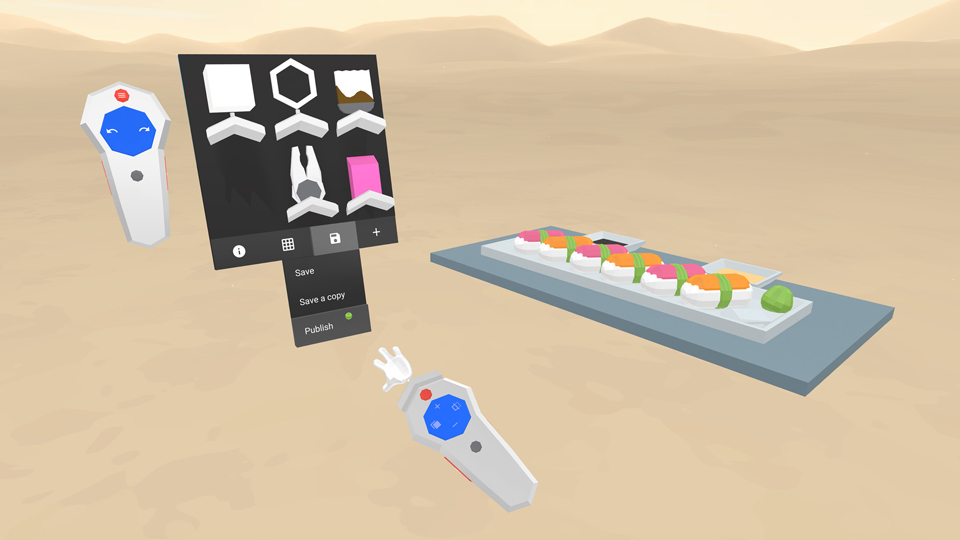
\includegraphics[width=0.487\linewidth]{figures/blocks_interface}\\
    (a)&(b)\\
    \end{tabular}
    \caption[Google Blocks]{Google Blocks.
    	  \textup{(a)} Model of an anglerfish created in Google Blocks.
			  \textup{(b)} Interface of Google Blocks. 
      \label{fig:blocks}}
\end{figure}
\chapter{System Description}
This chapter will give a description of the VR sketch-based modelling software, named SketchMeshVR, that was developed as part of this thesis. The software aims to provide users with a simple and intuitive sketch-based 3D modelling tool within a VR environment. Specifically the software is developed for use with the Oculus Rift including one Touch controller. Compared to the VR modelling software that was discussed in Section ~\ref{}\todo{insert section 3d modelling in vr} our system provides a novel method for creating 3D models. Whereas the existing modelling tools utilize volumetric brushes or predefined 3D shapes, our tool lets the user define the outline of a 3D shape and then fills in the inside of the outline. 

\section{Algorithms}
Algorithmically, SketchMeshVR largely follows FiberMesh by \cite{Nealen2007}. Similar to FiberMesh, users can draw strokes that define the 3D mesh surface, and these drawn strokes stay on the model surface to later function as deformation handles. Users can create an initial mesh, cut parts of the mesh, create extrusions, add and remove additional control curves and deform control curves on the mesh. Unlike in FiberMesh, SketchMeshVR does not give users the option to choose between smooth and sharp constraint curves and instead all curves are treated as smooth. The functionality to create tunnels through meshes is also not present in SketchMeshVR.  

SketchMeshVR is built inside the framework of libigl \cite{Jacobson2017} and uses Oculus C++ SDK in order to display everything on the Oculus Rift. The standard overlay menu that is included in libigl is disabled since the concept of overlays does not port well to the VR setting. Overlays are displayed too close to the eye making it very difficult for the eye to focus on them, which results in a highly unpleasant user experience. 

The system is multithreaded such that the VR display keeps on being updated while the mesh computations are being executed. When multithreading is not enabled the screen will freeze during the mesh computations, and therefore will stop updating when the user moves his head, breaking immersion and likely inducing motion sickness. 

Due to the direct availability of the actual 3D coordinates, some changes were made in comparison to the non-VR version. 
Whereas the non-VR version in drawing mode starts by converting mouse positions to screen coordinates and then unprojects these to 3D coordinates with a z-value of 0, SketchMeshVR takes the actual 3D coordinates and only projects them to 2D to allow triangulation. 
In the non-VR case, adding control curves on the mesh and later removing them is done by unprojecting the screen coordinates onto the mesh in order to get 3D positions and decide where the user wanted to add/remove a curve. In VR, instead of unprojecting the screen coordinates of the hand or taking the direct hand coordinates, we cast a ray from the hand position in the direction that the controller is being held. This intersection between this ray and the mesh is then used as the final 3D position for adding/removal.
When cutting in the non-VR program, the drawn stroke is interpreted purely in 2D. In order to create a loop on the front and back of the mesh surface, it is checked what edges are crossed (in 2D) by a line segment between two consecutive stroke points. Since the same 2D points are used for creating a surface path on the backside of the mesh, this results in perpendicular cuts (meaning that the "cutting knife" always goes perpendicular through the screen, and never at an angle). On the other hand, when cutting in VR we take the coordinates of both the first and second intersection between the cutting ray and the mesh. By doing this, we enable the possibility for the user to cut the mesh diagonally. In order to check which edges are crossed by the stroke segments, we find intersections between edges and the plane that is formed by the two points that make up the stroke segment and the position of the hand at the time of drawing that stroke segment. If an edge is intersected within its range, we know that the stroke segment crosses that edge. The surface path for the extrusion base is created in a similar fashion, except that only the first hit between ray and mesh is used. One problem that arises due to the fact that we're using 3D intersection points between the cutting ray and the mesh, is that we cannot easily derive the start and end points of the cutting stroke. These points are the final point outside of the mesh before we start drawing on top of the mesh and the first point outside of the mesh after drawing on top of the mesh respectively. \todo{probably include a drawing of this} We need these points in order to be able to find the mesh boundary edges that we need to cross to wrap the surface path around to the backside of the mesh. As mentioned before, in the non-VR case we simply use 2D coordinates based off the screen coordinates of the mouse pointer. In VR we cannot take the position of the controller as the user is likely cutting from a distance. What we've done in order to determine the start and end point is storing the controller position and direction for every sampled point that does not intersect the mesh. Then when the user releases the controller buttons after drawing  the cut stroke, we take these positions and directions and along these rays find the two points that are closest to the first and last point drawn onto the mesh. Under normal circumstances this will then give the two points outside of the mesh that are closest to the first and final cutting stroke points on the mesh. This method does however somewhat restrict the user in their freedom on how to draw the cut stroke. If the user holds his hand close to the mesh when starting the cut stroke, it is possible that the closest point to the initial on-mesh point actually is projected onto the mesh. This will make it impossible to create a looped surface path over the mesh. If this happens, a beep will sound and the cut stroke will be shown in black, allowing the user to try again.  \todo{probably include image}

Drawing the extrusion silhouette in VR is significantly different from the way it is done in non-VR. When defining the silhouette stroke in non-VR, the user first has to rotate the mesh such that it is looked at from a side view. Only then can the user sensefully specify the shape and depth of the extrusion silhouette, since we cannot gain any depth information from a frontal view. In VR on the other hand, we know the actual 3D positions of the controller and can therefore directly specify the extrusion silhouette in the frontal view. If the user prefers to do this from a side view instead (to get additional visual feedback about the silhouette depth on top of the tactile feedback), this is also possible.
Finally \todo{pull}

\section{User Interface}
For the user interface in virtual reality it was important to keep the controls for all actions very intuitive. Unlike the VR 3D modelling programs that were discussed in the previous work section\todo{put a ref to the specific section here}, SketchMeshVR does not have any menus in its interface. Instead all functionality in the program can be used with just the right Touch controller (in future versions the user should be able to choose whether to use the left or right controller as the primary one). To simplify orientating the user's hand in the scene, a sphere is displayed at the location of the right Touch controller, together with a ray from the hand following the orientation of the controller. When the user is in draw or pull mode or is drawing the extrusion silhouette, the ray disappears and only the hand sphere shows. This is done in order to emphasize that the actual position of the hand is used to draw a stroke, instead of the intersection points of the ray and mesh.

Compared to drawing strokes with a mouse on a PC screen (which happens purely in a 2D plane), drawing strokes in virtual reality with the Oculus Touch controller allows the user to draw strokes directly in 3D. In SketchMeshVR we made use of this advantage whenever possible. \todo{TEST DRAWING IN YZ PLANE (BUT NOT FULLY PERPENDICULAR)} However, when the user draws the stroke that is used to create the initial mesh, the software does assume that the stroke is drawn mostly on the plane that the user is looking at. This is due to the fact that the drawn points will be projected to this 2D plane before they are triangulated. Subsequent cutting or extrusion operations do not have to be made in the plane that is being viewed, as for these actions the actual 3D positions of the drawn points are used. 

\todo{position touch controller image}
To create an initial mesh, the user has to simultaneously press and hold the grip and trigger buttons while drawing a stroke in the air and subsequently release both when the stroke is finished. If the drawn stroke results in a non-edge manifold mesh (for example if the stroke intersects itself), a beep will sound and the stroke is displayed in black. Otherwise the created mesh will be shown, with the originally drawn stroke overlayed. 

In order to deform the mesh, a user can drag on all present mesh curves. The user can toggle between drawing and deformation mode by pressing the B button. Upon startup draw mode is selected. To perform the dragging, the user has to simultaneously press and hold down the grip and trigger buttons while his hand is close to the curve vertex that he wants to pull to a new position. Then while still pressing the grip and trigger buttons, the user needs to move his hand to the desired new position, and release both buttons when the desired result is achieved. The new vertex position is interpreted directly as the 3D position of the Touch controller, therefore also allowing deformation outside of the viewing plane (as compared to the non-VR version, which only allows in-plane deformation). 

The combination of grip and trigger buttons was chosen for these actions as they most resemble the feeling of holding a pencil and grabbing something in order to pull on it. 

To add extra control curves to an existing mesh, the user has to press and hold the trigger button while drawing the stroke onto the mesh. All points that are outside of the mesh will be ignored and will not be added to the control curve. 

In order to remove control curves (all except for the curve that created the initial mesh), the user can toggle from stroke adding mode to stroke removal mode by pressing down the right thumbstick. Upon startup the stroke adding mode is selected. 
\todo{say something about ray mesh intersection for both add and remove}

We decided to map the trigger button to the functions of adding and removing control curves since this feels like a natural way to select objects (removal) and to highlight areas (addition).

Finally with the B button the user can switch between cut and extrusion modes. Upon startup the toggle is set to cutting mode, which allows the user to cut off parts of the existing mesh. To make a cut the user has to first point the laser ray to somewhere outside of the mesh, and then while holding down the grip button draw the cutting stroke over the mesh and finally releasing somewhere outside of the mesh again. In order to minimize unwanted behaviour, the user's hand should be a distance of approximately the mesh diagonal away from the mesh when performing a cut action. If anything went wrong during the cutting procedure, the drawn stroke will show on the mesh in black and a beep will sound. 
When in extrusion mode, the user has to start on the mesh and then while pressing the grip button has to draw the extrusion base on the mesh and release the button when the stroke is complete. Just like in the control curve addition mode, any points that are drawn outside of the mesh will be ignored. To ensure a correct functioning of the algorithm, the drawn base stroke has to have at least one vertex on its interior. Then to complete the extrusion, the user has to draw the extrusion silhouette stroke that will define the height of the extrusion. When drawing this stroke, the user has to press and hold the grip button again but this time the actual position of the Touch controller will be used instead of the ray-mesh intersection point. Releasing the grip button will start the extrusion computations.

When pressing only the grip button, the hand often naturally assumes a position that resembles the way we symbolize pistols with our hands. Intuitively this maps to the concept of shooting a laser ray from your hand, which would be a sensible tool to cut a mesh with. For the case of extrusion we can argue something similar, as part of the mesh topology is also cut away. For this reason the grip button was mapped to the cut and extrude modes.

\begin{figure}[!h]
    \centering
    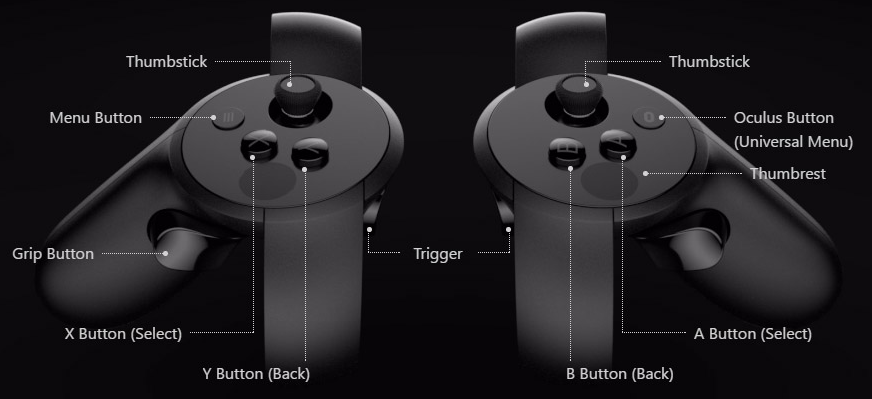
\includegraphics[width=0.7260\linewidth]{figures/touch_controllers}\\
    \caption[Oculus Touch controllers]{Button layout of the Oculus Touch controllers.
      \label{fig:touch_controller}}
\end{figure}


\begin{table}
    \centering
    \ra{1.1}
    \begin{tabular}{lp{0.4\linewidth}}
    \toprule
    \emph{Quant.} & \emph{Ingredient}\\
    \midrule
		200g &Wei{\ss}mehl\\
		1/4  &Packung Frischhefe\\
		4EL  &lauwarme Milch\\
		4EL  &�l\\
		1TL  &Zucker\\
		1TL  &Salz\\
		&lauwarmes Wasser\\
    \bottomrule
    \end{tabular}
    \caption[Flammkuchenteig]{Flammkuchenteig. The ingredients have to be carefully chosen.\label{tab:mytable}}
\end{table}



\chapter{Results}
\label{chap:results}

\section{Interface}
As mentioned in the previous chapter, SketchMeshVR does not make use of any menus and instead solely relies on different combinations of button presses to differentiate between the multiple available modelling actions. This does require more effort from the user in order to keep track of the selected editing modes, but at the same time keeps the interface cleaner. In order to guide the user when drawing strokes, SketchMeshVR provides visual feedback on the positions that will be used to create a stroke. In case of the drawing and curve deformation modes this means that the user sees the position controller and in case of all other modes the user will see the position controller plus a ray shooting from it (the ray ends at any intersections it has with the scene). Figures~\ref{fig:interface}(a) and (b) show what this looks like.

\begin{figure}[!h]
    \centering
    \setlength{\tabcolsep}{0.0130\linewidth}
    \begin{tabular}{@{}cc@{}}
    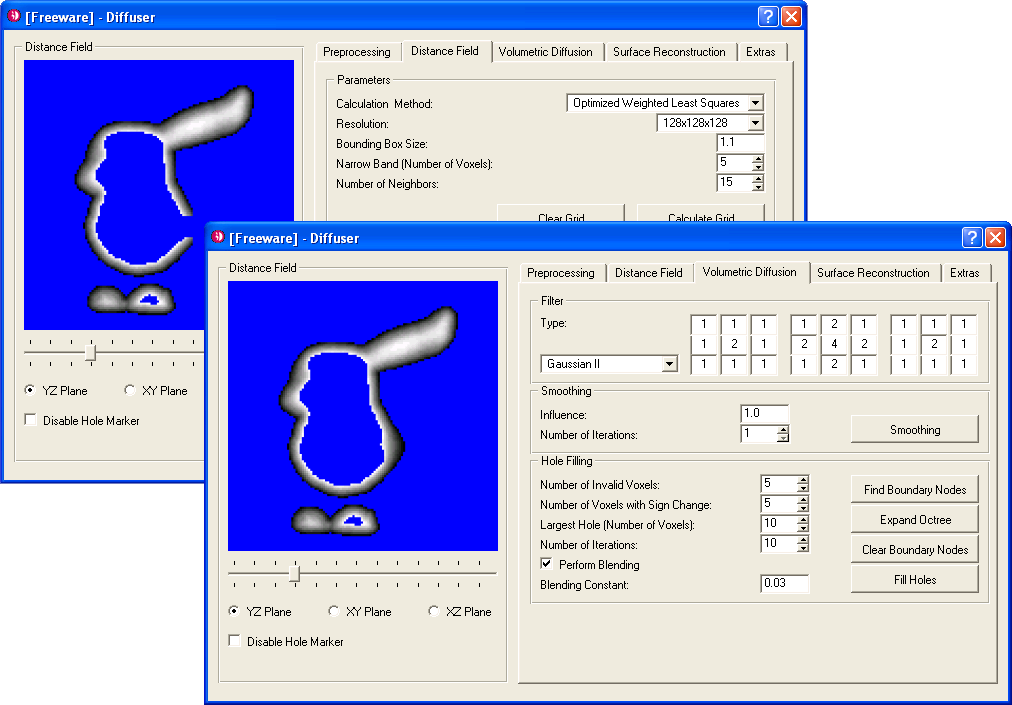
\includegraphics[width=0.3\linewidth]{figures/voldiff_ui}&
  	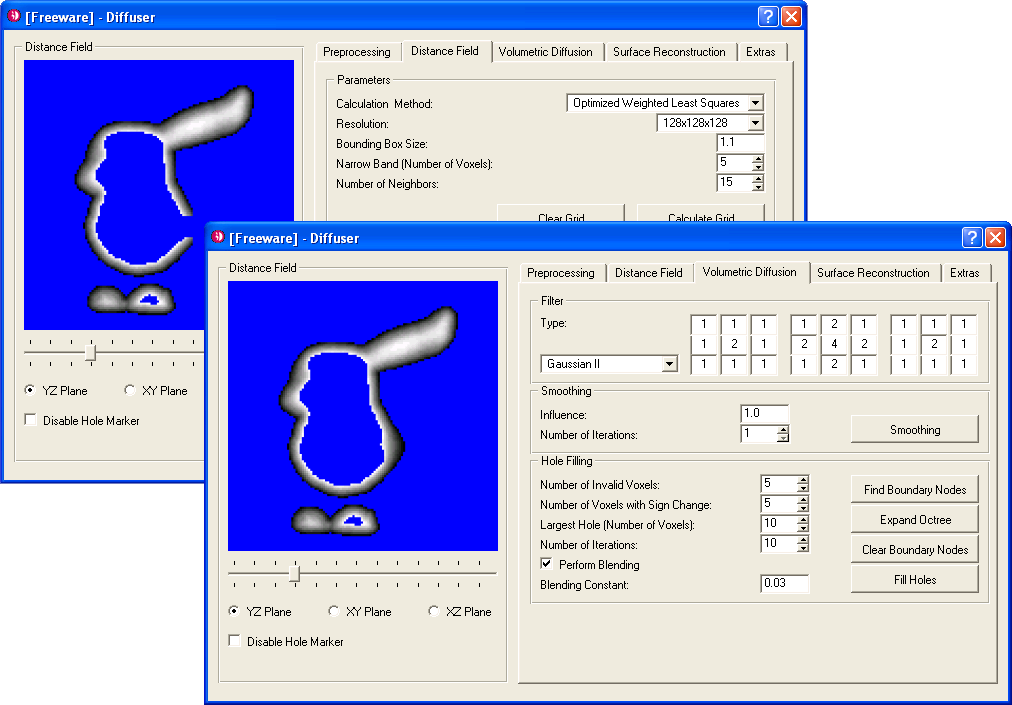
\includegraphics[width=0.3\linewidth]{figures/voldiff_ui}\\
    (a)&(b)\\
    \end{tabular}
    \caption[SketchMeshVR interface]{SketchMeshVR interface.
    	  \textup{(a)} Controller reference point that is displayed in drawing and deformation mode.
			  \textup{(b)} Controller and ray reference that are displayed in all other editing modes. 
      \label{fig:interface}}
\end{figure}
 
\section{User review}

\textcolor{red}{TODO:}
\begin{itemize}
\item mention test users' prior experience with 3D modelling and VR
\item explain test setup: asking users to recreate an example model both in VR \& non-VR version of program
\item summarize any comments they have on the test/experience
\item what did they think of ease of learning/modelling?
\item Is there a difference in efficiency between modelling in VR or non-VR?
\item show side-by-side comparisons of example model and user recreations
\end{itemize}


\begin{figure}[!h]
    \centering
    \setlength{\tabcolsep}{0.0130\linewidth}
    \begin{tabular}{@{}ccc@{}}
    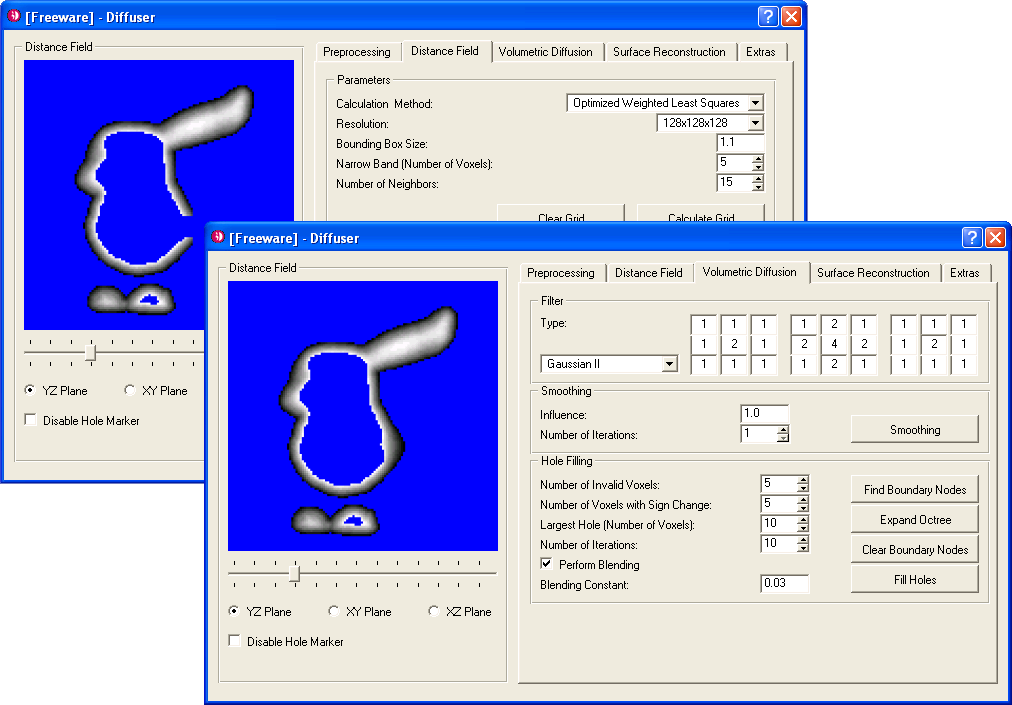
\includegraphics[width=0.3\linewidth]{figures/voldiff_ui}&
  	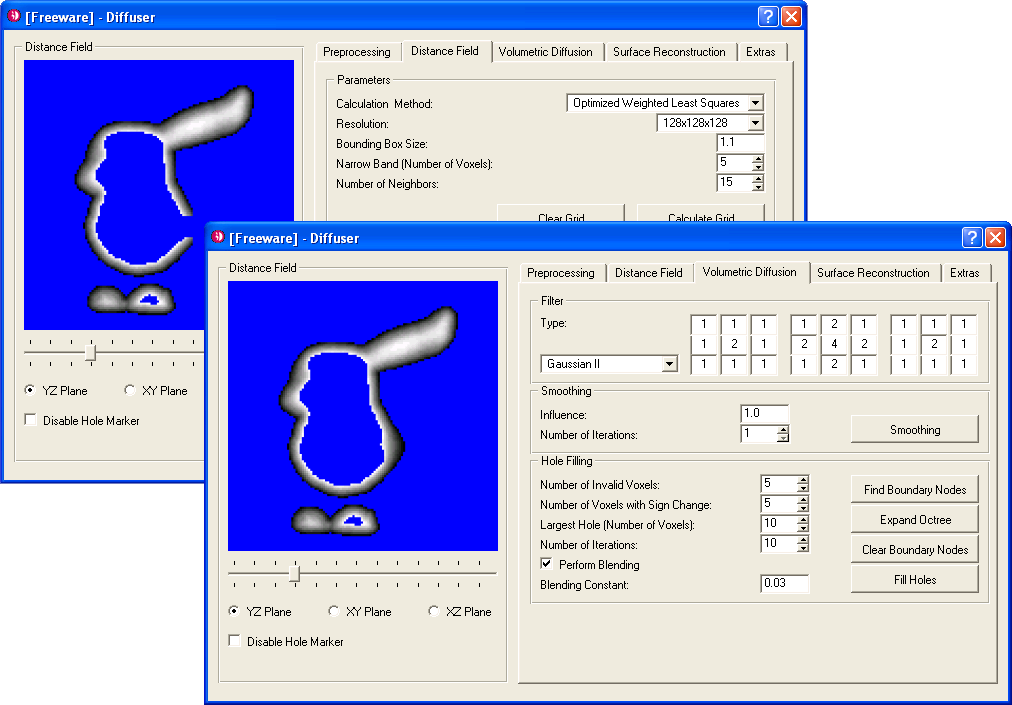
\includegraphics[width=0.3\linewidth]{figures/voldiff_ui}&
  	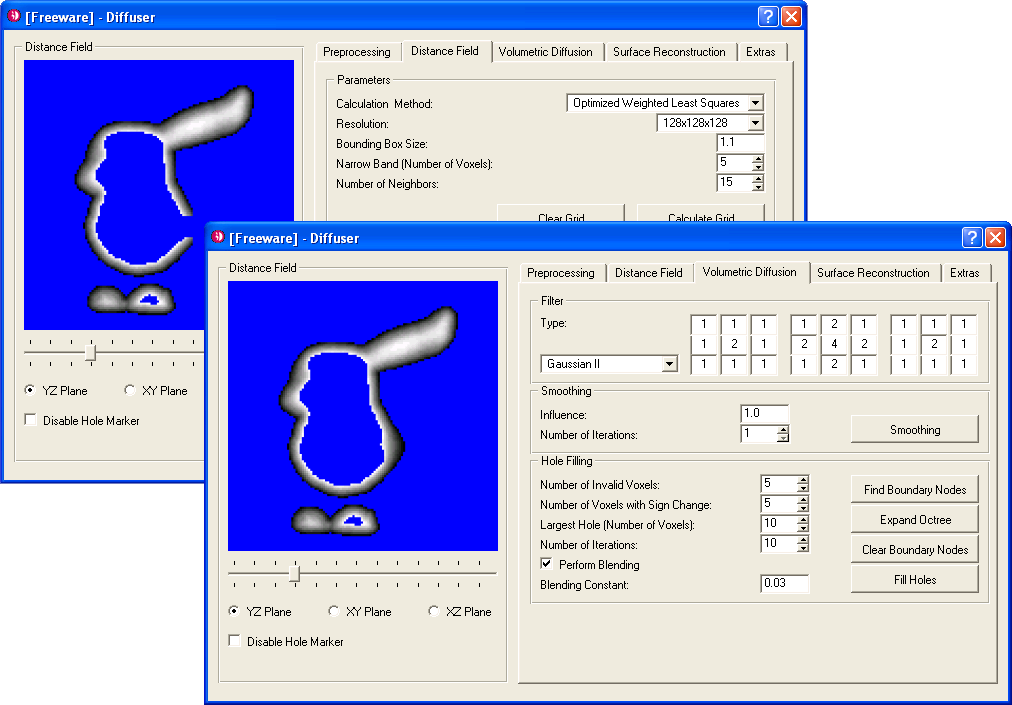
\includegraphics[width=0.3\linewidth]{figures/voldiff_ui}\\

    (a)&(b)&(c)\\
    \end{tabular}
    \caption[SketchMeshVR teddy model]{SketchMeshVR recreating models.
    	  \textup{(a)} Example simplified mesh of a teddy bear.
	  \textup{(b)} Resulting recreated model made in VR  (took X seconds to complete).
	  \textup{(c)} Resulting recreated model made in non-VR (took Y seconds to complete).
      \label{fig:recreate_teddy}}
\end{figure}
\todo{Fill in taken seconds in caption}


\begin{figure}[!h]
    \centering
    \setlength{\tabcolsep}{0.0130\linewidth}
    \begin{tabular}{@{}ccc@{}}
    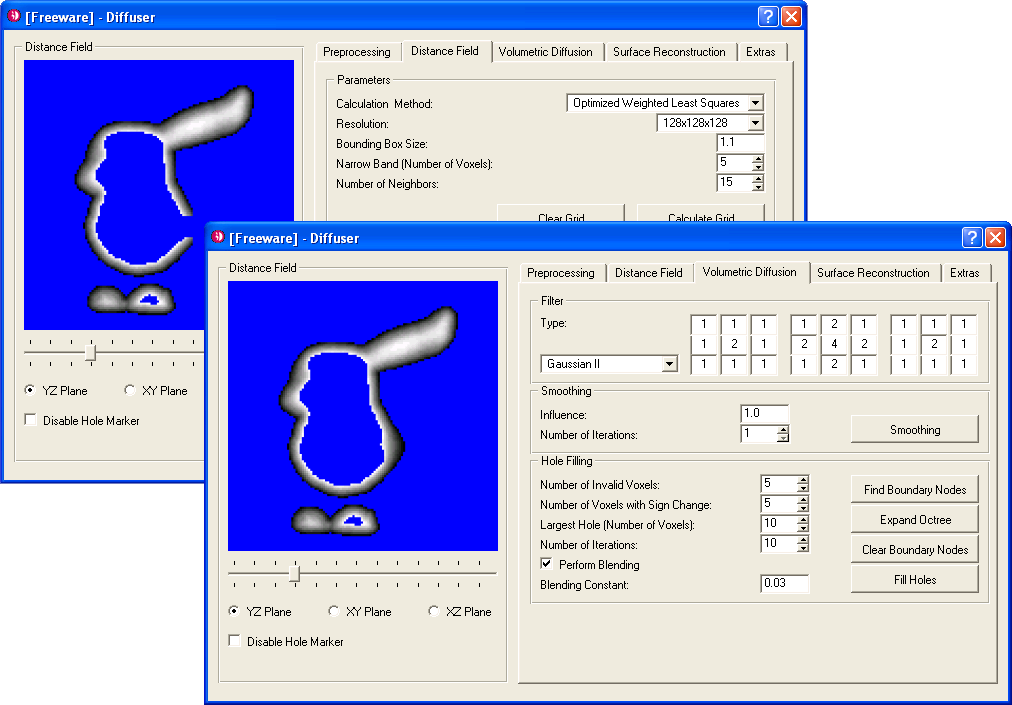
\includegraphics[width=0.3\linewidth]{figures/voldiff_ui}&
  	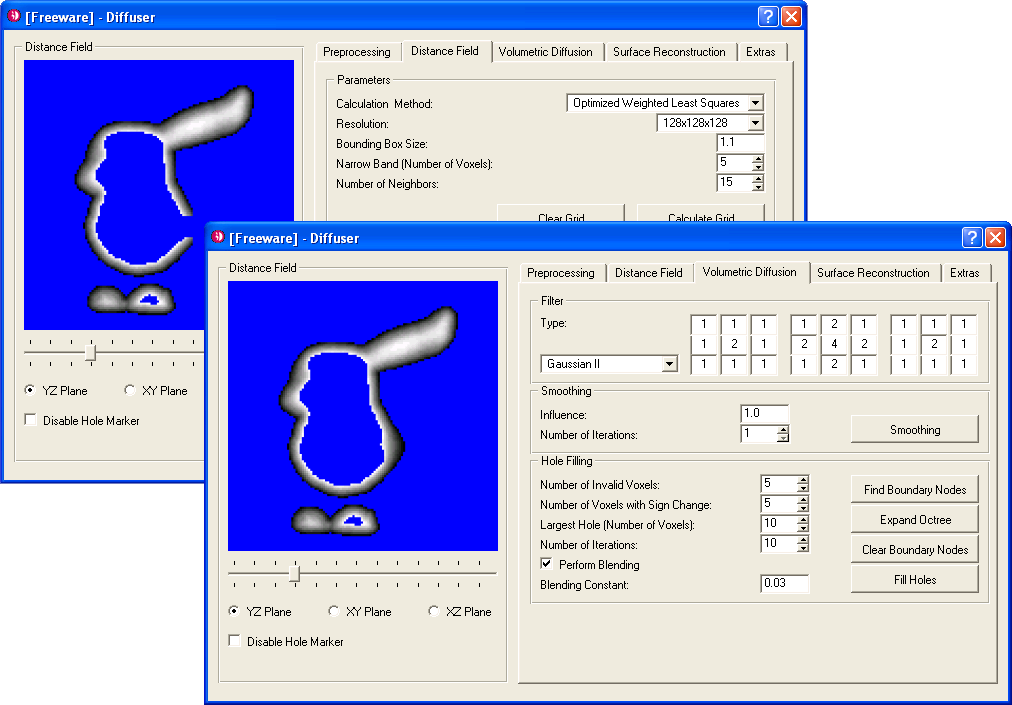
\includegraphics[width=0.3\linewidth]{figures/voldiff_ui}&
  	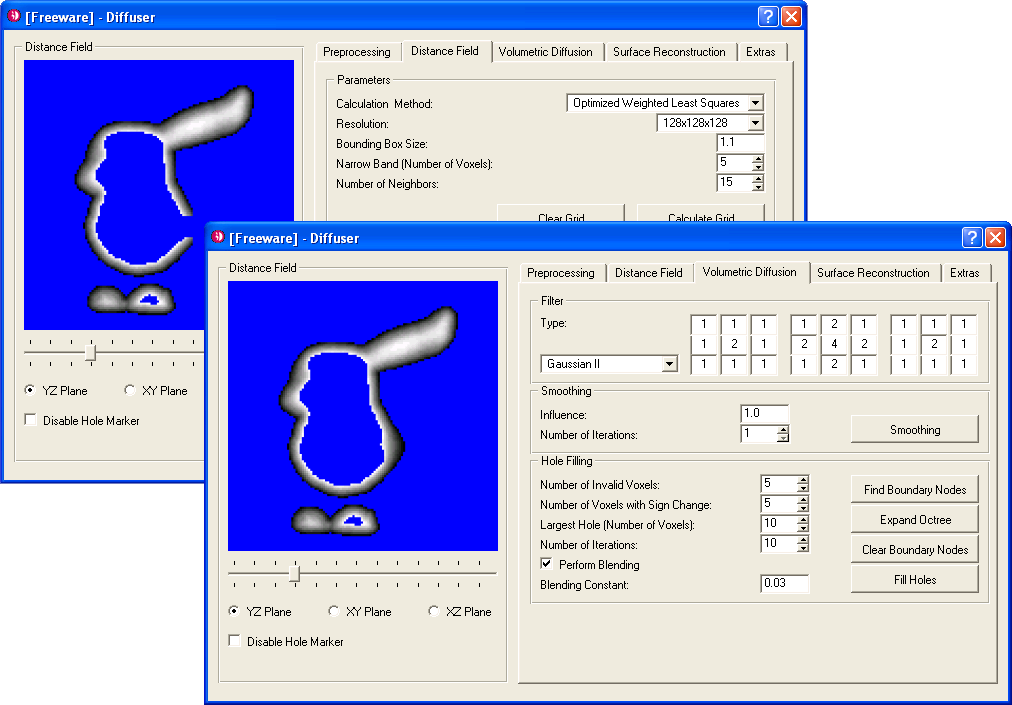
\includegraphics[width=0.3\linewidth]{figures/voldiff_ui}\\

    (a)&(b)&(c)\\
    \end{tabular}
    \caption[SketchMeshVR dolphin model]{SketchMeshVR recreating models.
    	  \textup{(a)} Example simplified mesh of a dolphin.
	  \textup{(b)} Resulting recreated model made in VR (took X seconds to complete).
	  \textup{(c)} Resulting recreated model made in non-VR (took Y seconds to complete).
      \label{fig:recreate_dolphin}}
\end{figure}
\todo{Fill in taken seconds in caption}
\chapter{Conclusion and Outlook}
\label{chap:conclusion}

\section{Future work}
The developed software still offers potential for future expansion and improvements. For instance, the software misses some of the useful tools that are present in other modeling software such as simple predefined shapes (like cubes or cylinders), mirroring and merging meshes. Using a second VR controller (e.g.\ the Oculus Touch controller) gives enough buttons to map these functions to, allowing us to implement them without the addition of menu, thus staying with the principle of "intuitive" hand gestures. Adding an extra controller also allows for the user to switch between smooth and sharp curve deformation. The functionality for this is embedded in the software, but is not mapped to any button because all buttons of the first controller are already occupied by other functions. 

Another functionality that would prove to be useful in many cases is the possibility to use blueprint images. When working with blueprint images, the user defines a series of different images of an object each taken from a different viewpoint. This allows them to trace these silhouettes from different angles and precisely recreate the object they want to model.

Additionally, the quality of the created meshes could greatly be improved by applying intermediate remeshing. As can be seen from the mesh examples, the triangle sizes differ greatly between triangles that are part of the initial created shape and triangles that are part of a subsequent cut surface or extruded part. This makes the appearance of the mesh rather chaotic and this could be avoided by remeshing every time a new surface is created. The purpose of the remeshing would be to make the edge lengths more uniform across the different parts of the mesh, resulting in a much more homogeneous mesh structure.

Final possibilities for improvements to the software lie in improving the interface. Implementing hand avatars for hand orientation instead of a simple sphere greatly increase the feeling of immersion. Furthermore, displaying the currently selected tool modes (for example cutting versus extrusion mode) is an addition that will greatly help the user in keeping track of the type of mood that is selected, especially when there is a lot of switching going on. This could be done either by including a HUD (head-up display), a distanced billboard or customized meshes for each tool as is done in Google Blocks (Figure~\ref{fig:blocks_tool} gives an example). Additionally enabling the user to navigate the mesh either with one of the thumbsticks or with hand gestures using the two controllers is a valuable extension that will improve the usability, especially for users who do not have a lot of space available to physically walk around the mesh. 

\begin{figure}[!h]
    \centering
    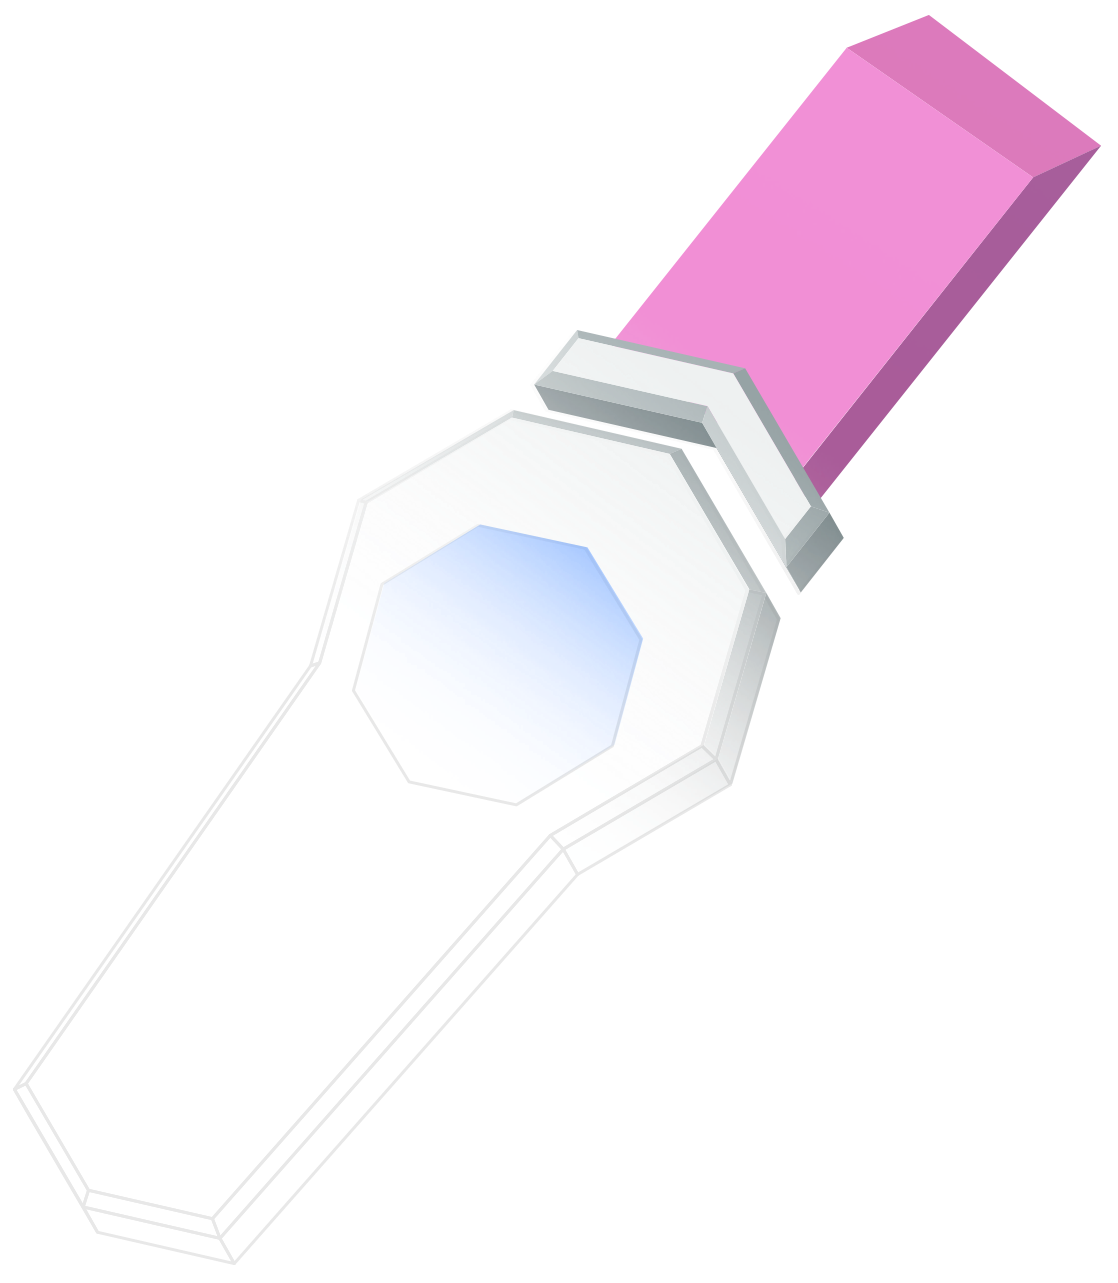
\includegraphics[width=0.3\linewidth]{figures/blocks_tool}\\
    \caption[Google Blocks tool avatars]{Google Blocks' customized hand avatar for the eraser mode.
      \label{fig:blocks_tool}}
\end{figure}

\section{Conclusion}
In this thesis we have presented a novel way of creating 3D models in virtual reality. Modeling 3D objects in VR in itself is not a novel concept, but to the best of our knowledge our software newly introduces the sketch-based 3D modeling paradigm to VR. Whereas other programs mostly work with volumetric brushes and tools to edit the created "clay-like" models, ours transfers the concept of sketch-based modeling to VR by letting the user define model silhouettes. Although volumetric brushes allow for more fine-grained control over the resulting model, we believe that our method provides a more accessible and effortless way of creating simple models. In our opinion, if the goal is to provide the user with an intuitive and uncomplicated way of creating 3D models in VR, SketchMeshVR is better suitable to do the task than other 3D modeling tools for VR like Google Blocks or Oculus Medium. 

We can conclude that virtual reality provides a very useful and powerful extension to traditional 3D modeling and that bringing the sketch-based paradigm to a VR setup makes it even more versatile. Users reported that directly working in 3D especially made out-of-plane editing operations a lot more intuitive as compared to performing these operations in a traditional PC and mouse setting.

The source code for SketchMeshVR (and also its non-VR version), along with instructions for installation can be found online at \url{https://github.com/FloorVerhoeven/SketchMeshVR}. 


% ---- END MAIN PART ----

\clearpage
\renewcommand*{\chapterpagestyle}{empty}

%\nocite{*}
\cleardoublepage
\phantomsection
\addcontentsline{toc}{chapter}{Bibliography}
\bibliography{testbib}

\end{document}
